\chapter{プロトタイピング}
\label{prototyping}
本研究では、「手指の変換表現」についての\ref{prototyping_concept_making}節のような動機を起点に「人馬一体感」のデザインが目的となり、修士作品《Grasp(er)》を制作した。ここでは、その過程にあるプロトタイピングについて説明する。
本章ではまず、それらのプロトタイプについて、「形状」、「マッピング」、「時間操作」、「ボール操作」の観点から分類する。その上で、これらのプロトタイピングを前の指標に照らし合わせた上で、それを具現化する表現が何であったかについて述べる。

\section{プロトタイプの分類}
修士作品の制作に至るまでに、2022年6月から2023年10月までの期間で、総計60パターンのバリエーション、並びに計6回のプロトタイプの展示を実施した。

プロトタイピング、並びに修士作品には、Tensorflowの開発グループがサンプルとして提供するhand-pose-detection\footnote{\url{https://github.com/tensorflow/tfjs-models/tree/master/hand-pose-detection}}を用いた。このモデルでは、手指の動きが下図\ref{fig:keypoints}に示す21個のキーポイントで表現される。こうしたキーポイントの情報をもとに、その配置や関係性といった構造、そしてそれをどのように表現するのか、といった点から変換表現について検討した。また、単に形を考えるだけでなく、どのようにマッピングさせるか、そしてどの時間の動きを用いるか等、さまざまな変換方法を検討した。先入観によって絞り込むことがないよう、このような探索空間の中で思いつく限り実装し、実際に体験することを通して判断するという姿勢でプロトタイピングをおこなった。

\begin{figure}[H]
  \centering
  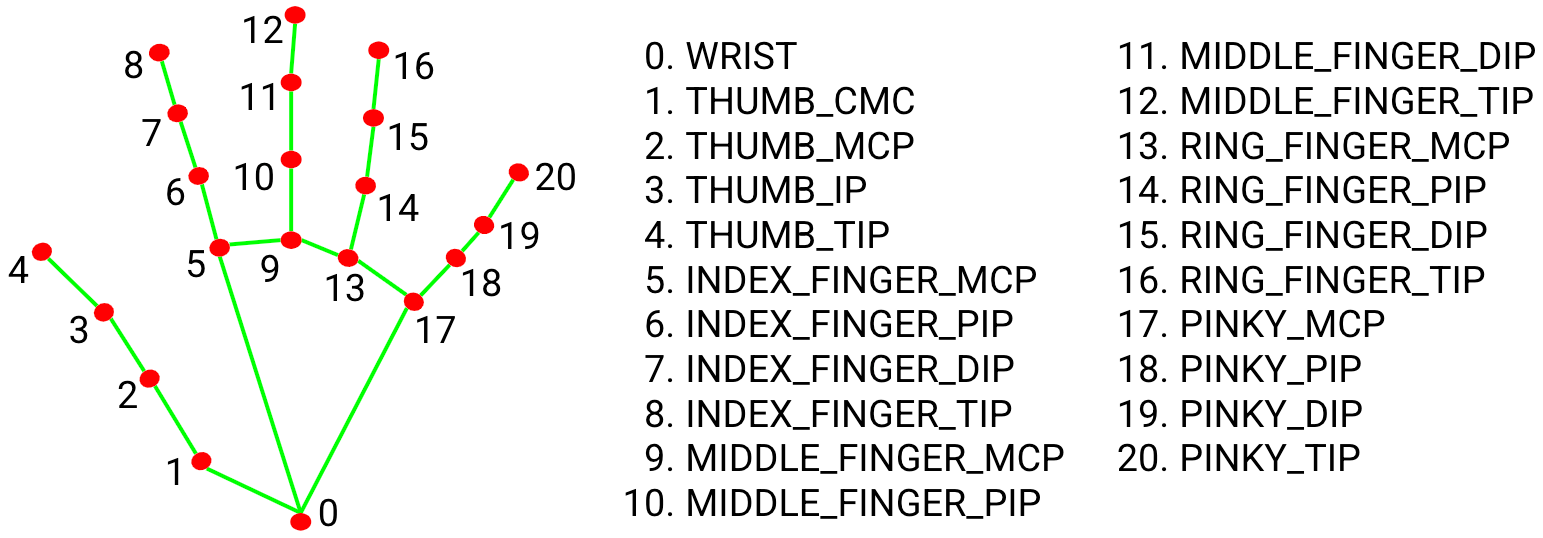
\includegraphics[width=15cm]{img/hand_keypoints.png}
  \caption{モデルを用いて表現されるキーポイント:hand-pose-detectionモデルのリポジトリより引用}
  \label{fig:keypoints}
\end{figure}

\subsection{形状}
形状については、指を1つのユニットとして捉えて、ユニット自体の形状やそれらをどのように関連づけるのかについて検討したもの、そうした枠組みとは無関係に制作したものとの2つに分類して説明する。
\subsection*{指をユニットと捉えたバリエーション}
キーポイントの情報を指ごとに分割して捉え、指一本の中で生じる動きを一つのユニットと捉えてバリエーションを展開した。以下の図\ref{fig:unit_valiation}に示す「ドット」や「ライン」は指のキーポイントを点群として離して出力するか、一つの線として繋げて表示するかの違いである。また、「円」、「くの字」、「クロス」などのバリエーションは、指先の\(y\)座標と指の付け根の\(y\)座標の差を評価して、ユニットの高さ(あるいは直径)が変化する。
\begin{figure}[H]
  \centering
  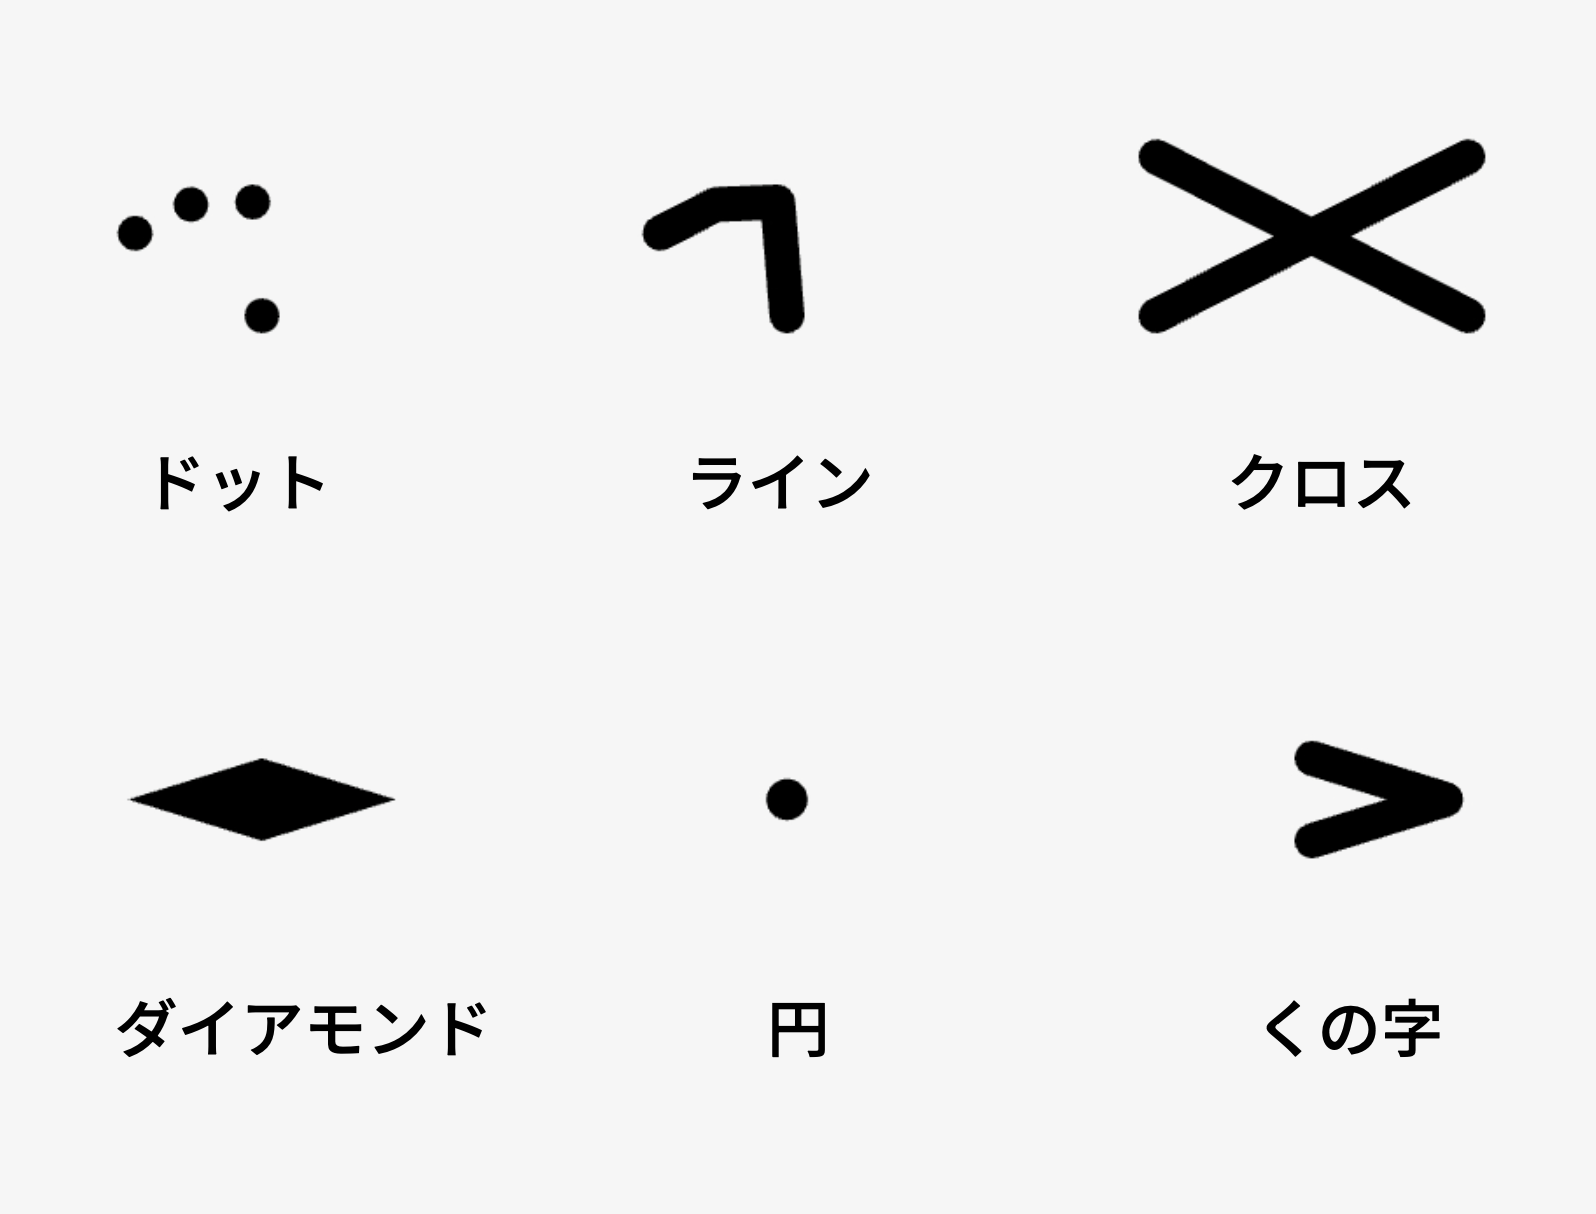
\includegraphics[width=10cm]{img/unit_valiation.png}
  \caption{ユニットのバリエーション}
  \label{fig:unit_valiation}
\end{figure}

また、これらユニットをいかに繋ぎ合わせて1つの形にするかについても探索を行なった(\ref{fig:connection_valiation})。以下は、同じ「くの字」のユニットについて、「並列に並べたもの」、「片手ずつ直列に繋ぎ、左右の同じ指の高さを結ぶ直線の傾きで回転をかけたもの」、「円形に繋げたもの」の3つのバリエーションである。(3枚画像を追加する)

\begin{figure}[H]
  \centering
  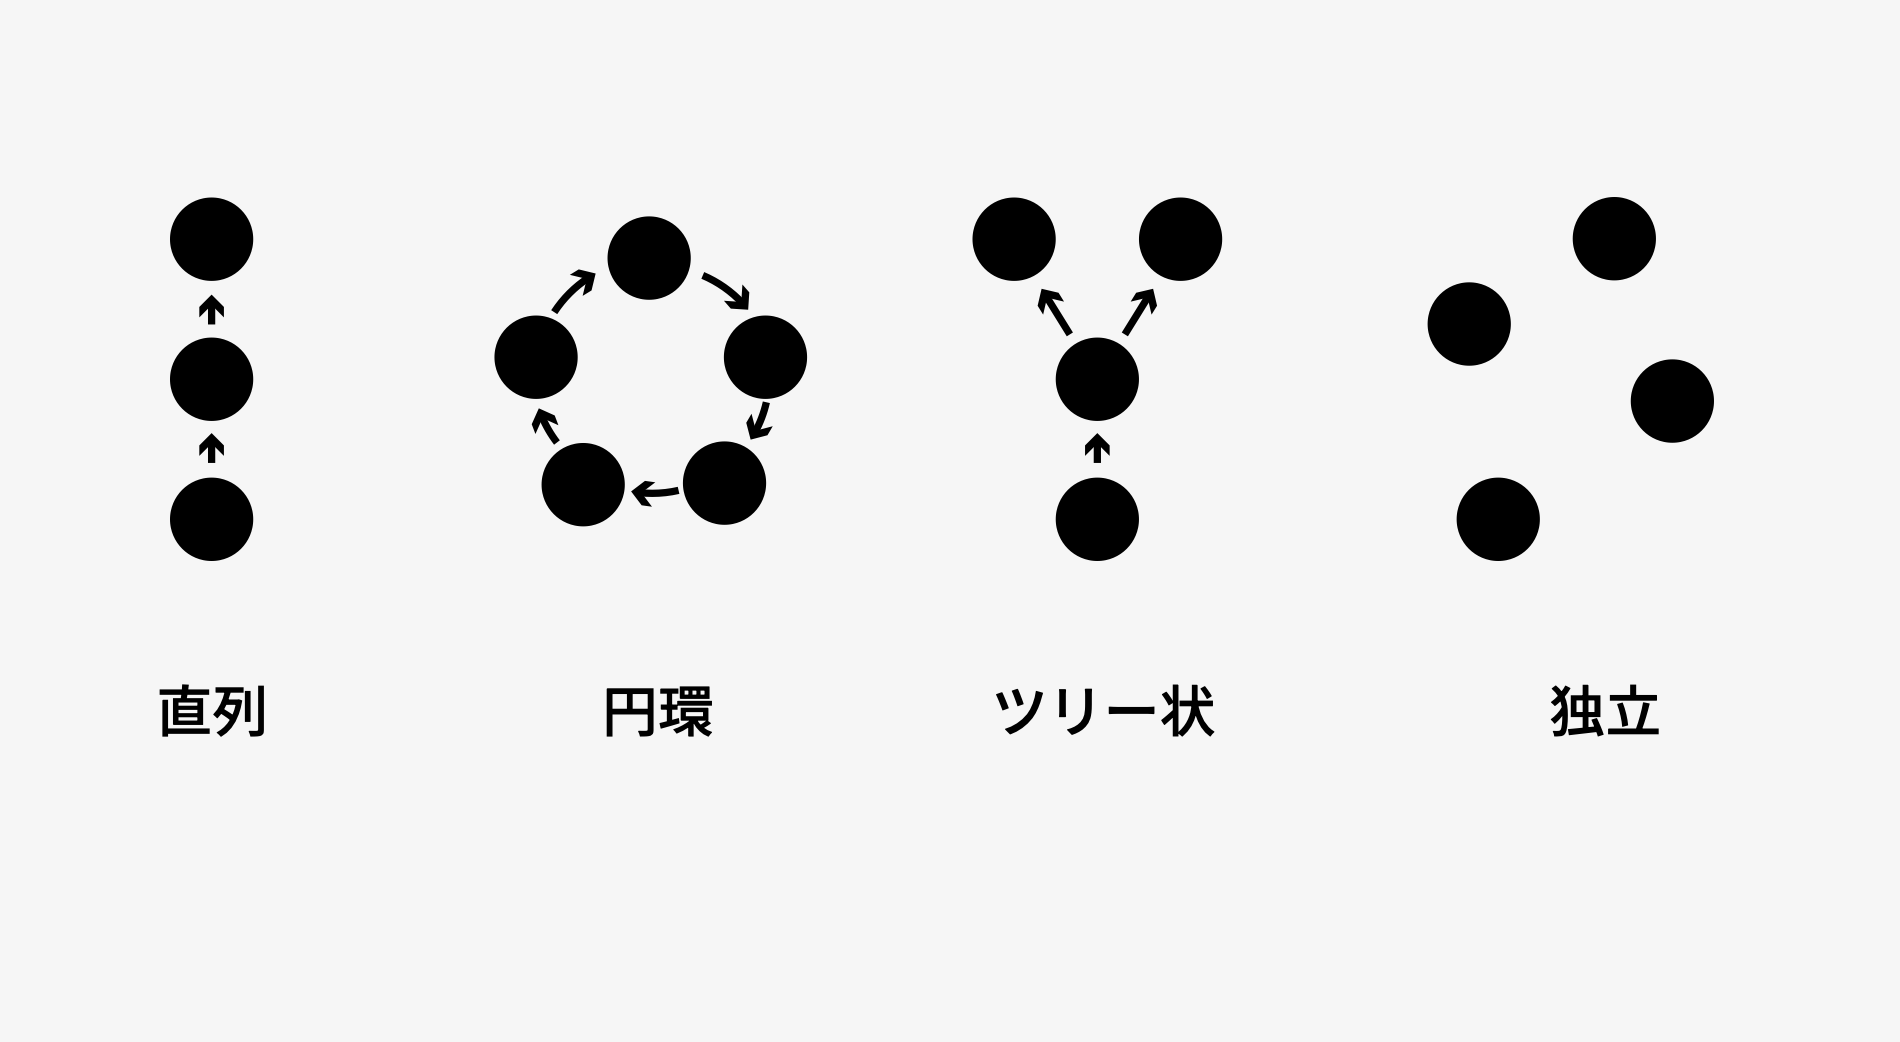
\includegraphics[width=10cm]{img/network.png}
  \caption{繋ぎ方のバリエーション}
  \label{fig:connection_valiation}
\end{figure}



\subsection*{指をユニットとしないバリエーション}
手指の動きを全て包み込む皮膜を「凸包(convex envelope)」のアルゴリズムを用いて実装したり、また指先と付け根の動きだけでなく、指の関節の開き具合を変数として、二等辺三角形の頂角の大きさが変化するバリエーションなどを作成した。

\subsection{マッピング}
マッピングについては、1つの動きが1箇所に対応しているものだけでなく、1つの動きを複数のパーツの動きへと複製したバリエーションなどを作成した。図\ref{fig:networked_finger}に示すプロトタイプ\footnote{\url{https://eee-handpose-playground.vercel.app/work/createNetworkedFingers}}では、指先をクリックすると5本ある指のうちのいずれかの動きを追従する指が、指先に追加されるものである。どの指が付け加わるかはランダムである。そのため指が新しく追加されるたびに、一本一本指を動かして、どこがその指に対応しているのかについて同定する必要がある。

またそのほかに、図\ref{fig:fractal_finger}に示すプロトタイプ\footnote{\url{https://eee-handpose-playground.vercel.app/work/fractalFingers}}は、フラクタル構造で指の動きを配置したバリエーションである。親指の先に人差し指の動きが複数分岐し、さらに人差し指の先から中指の動きが複数分岐して配置される。

\begin{figure}[htbp]
  \begin{minipage}[b]{0.5\linewidth}
    \centering
    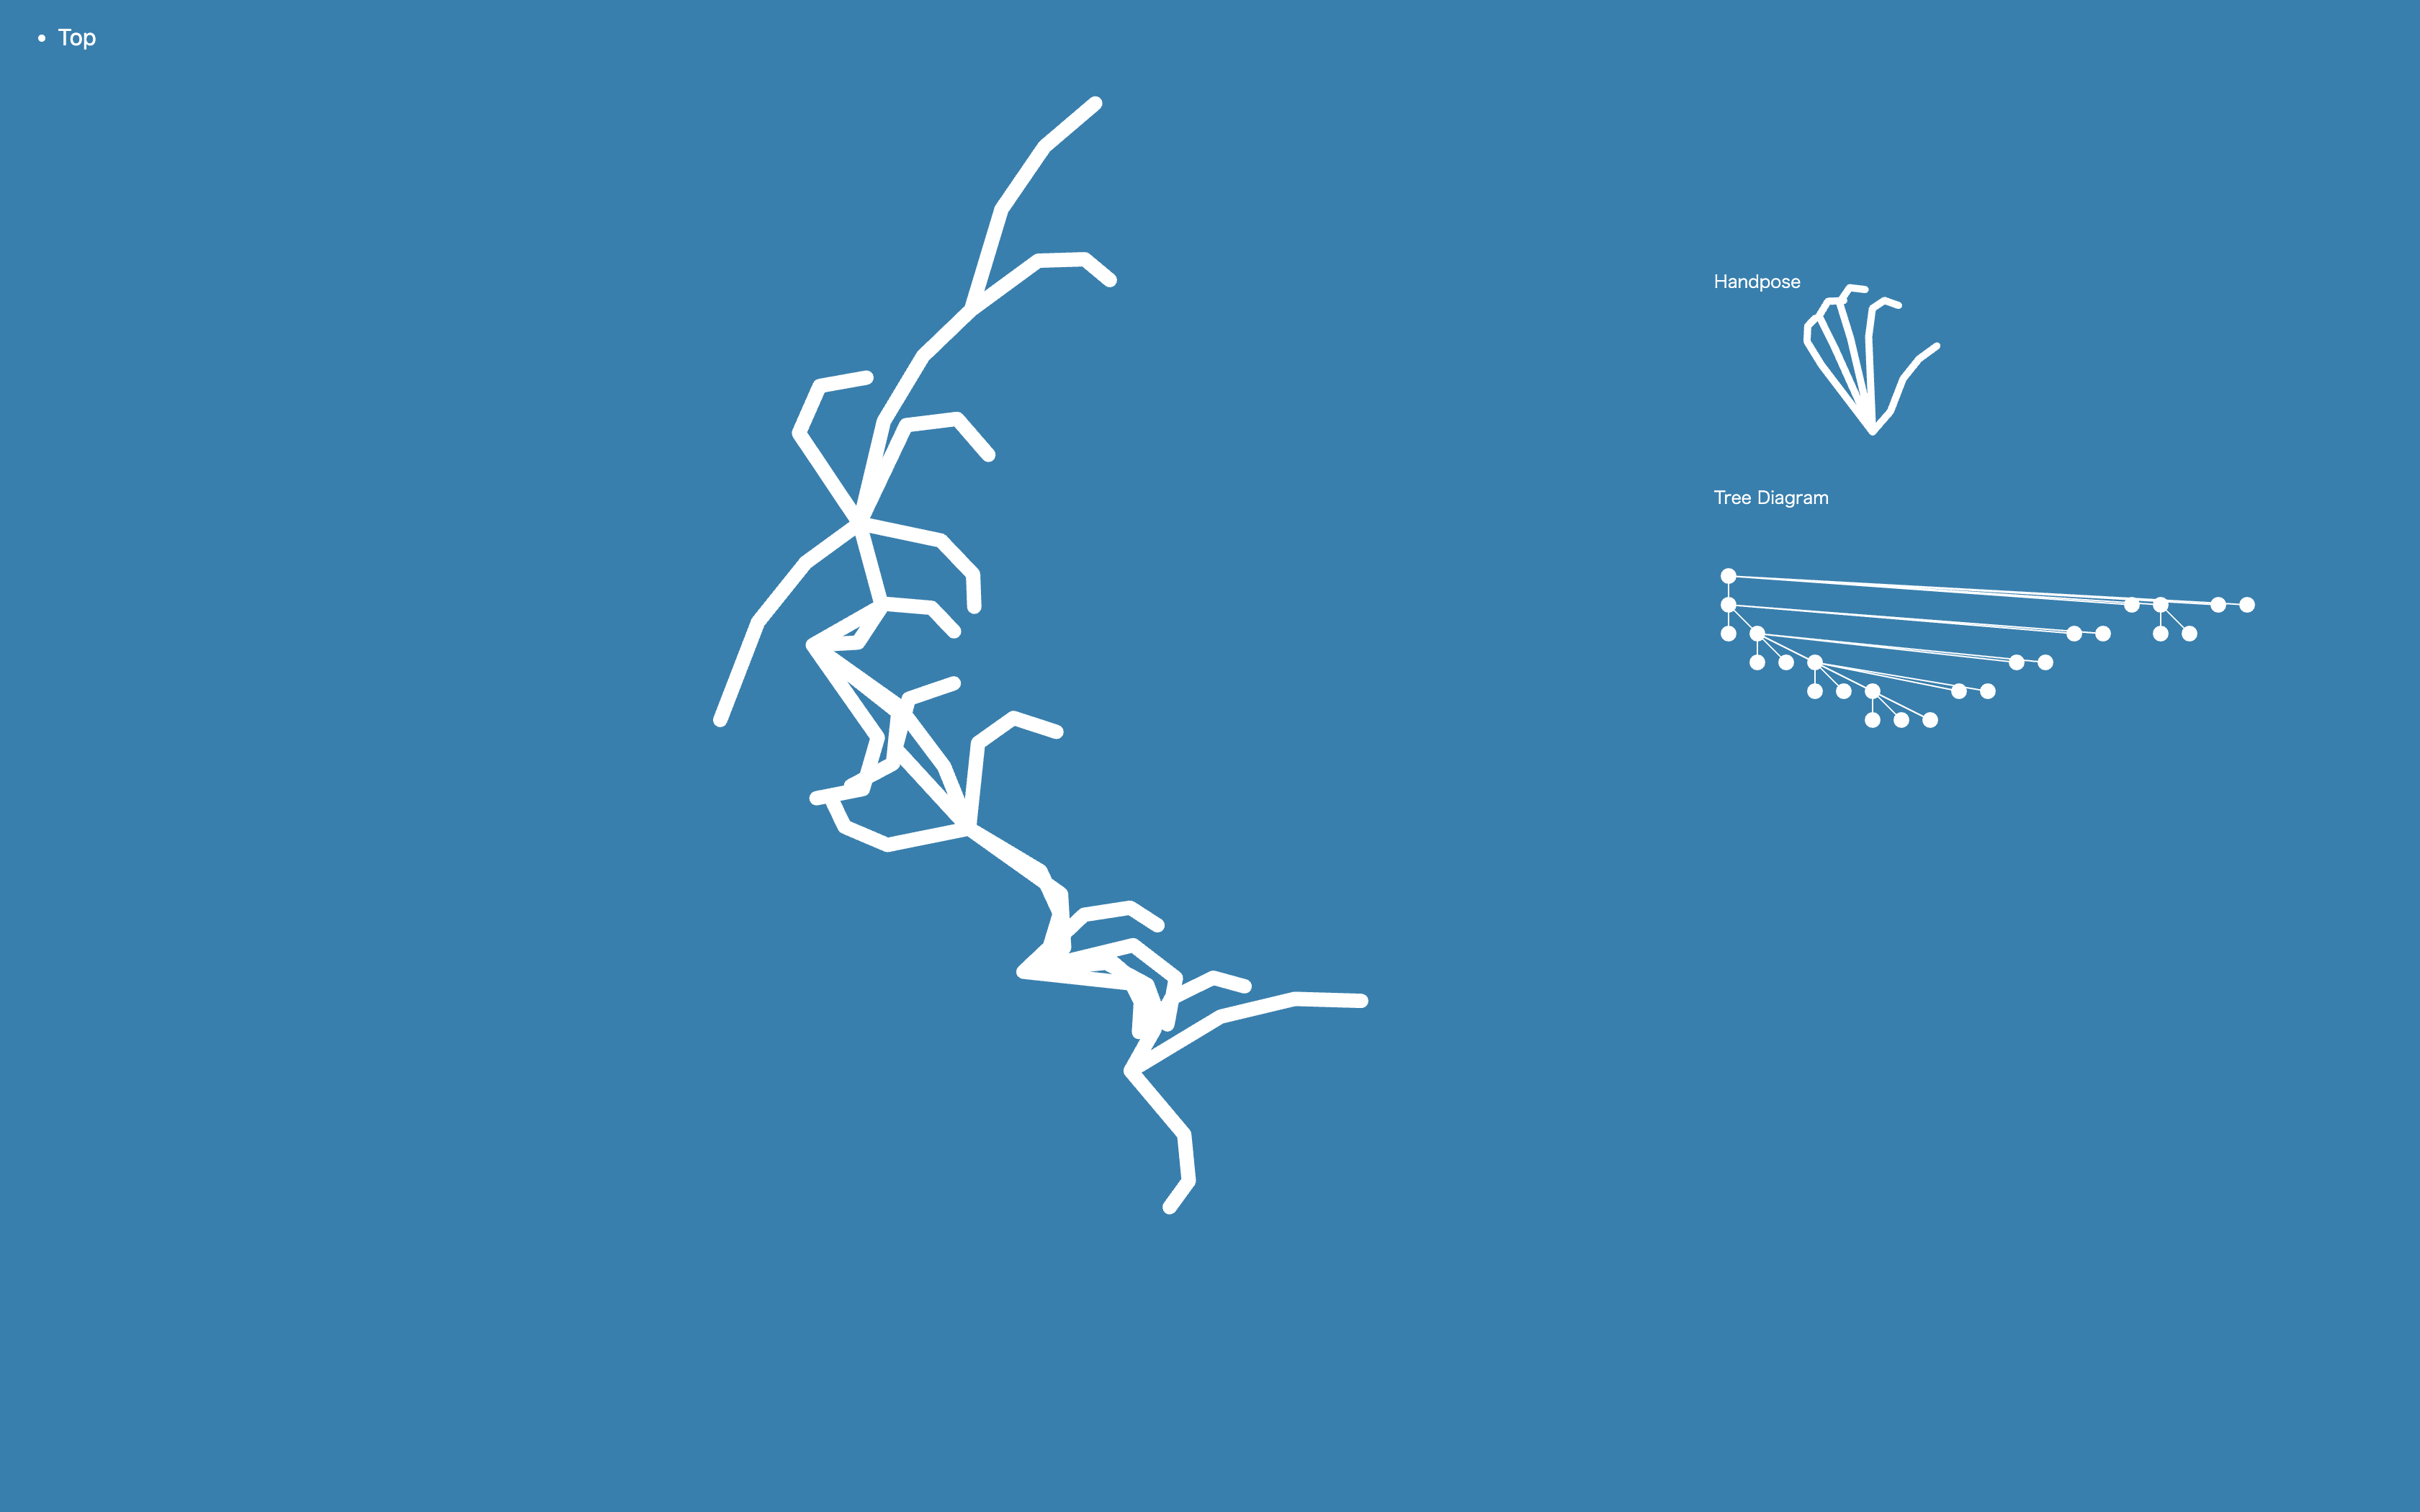
\includegraphics[keepaspectratio, width=7cm]{img/networked_finger.png}
    \caption{Networked Finger}
    \label{fig:networked_finger}
  \end{minipage}
  \begin{minipage}[b]{0.5\linewidth}
    \centering
    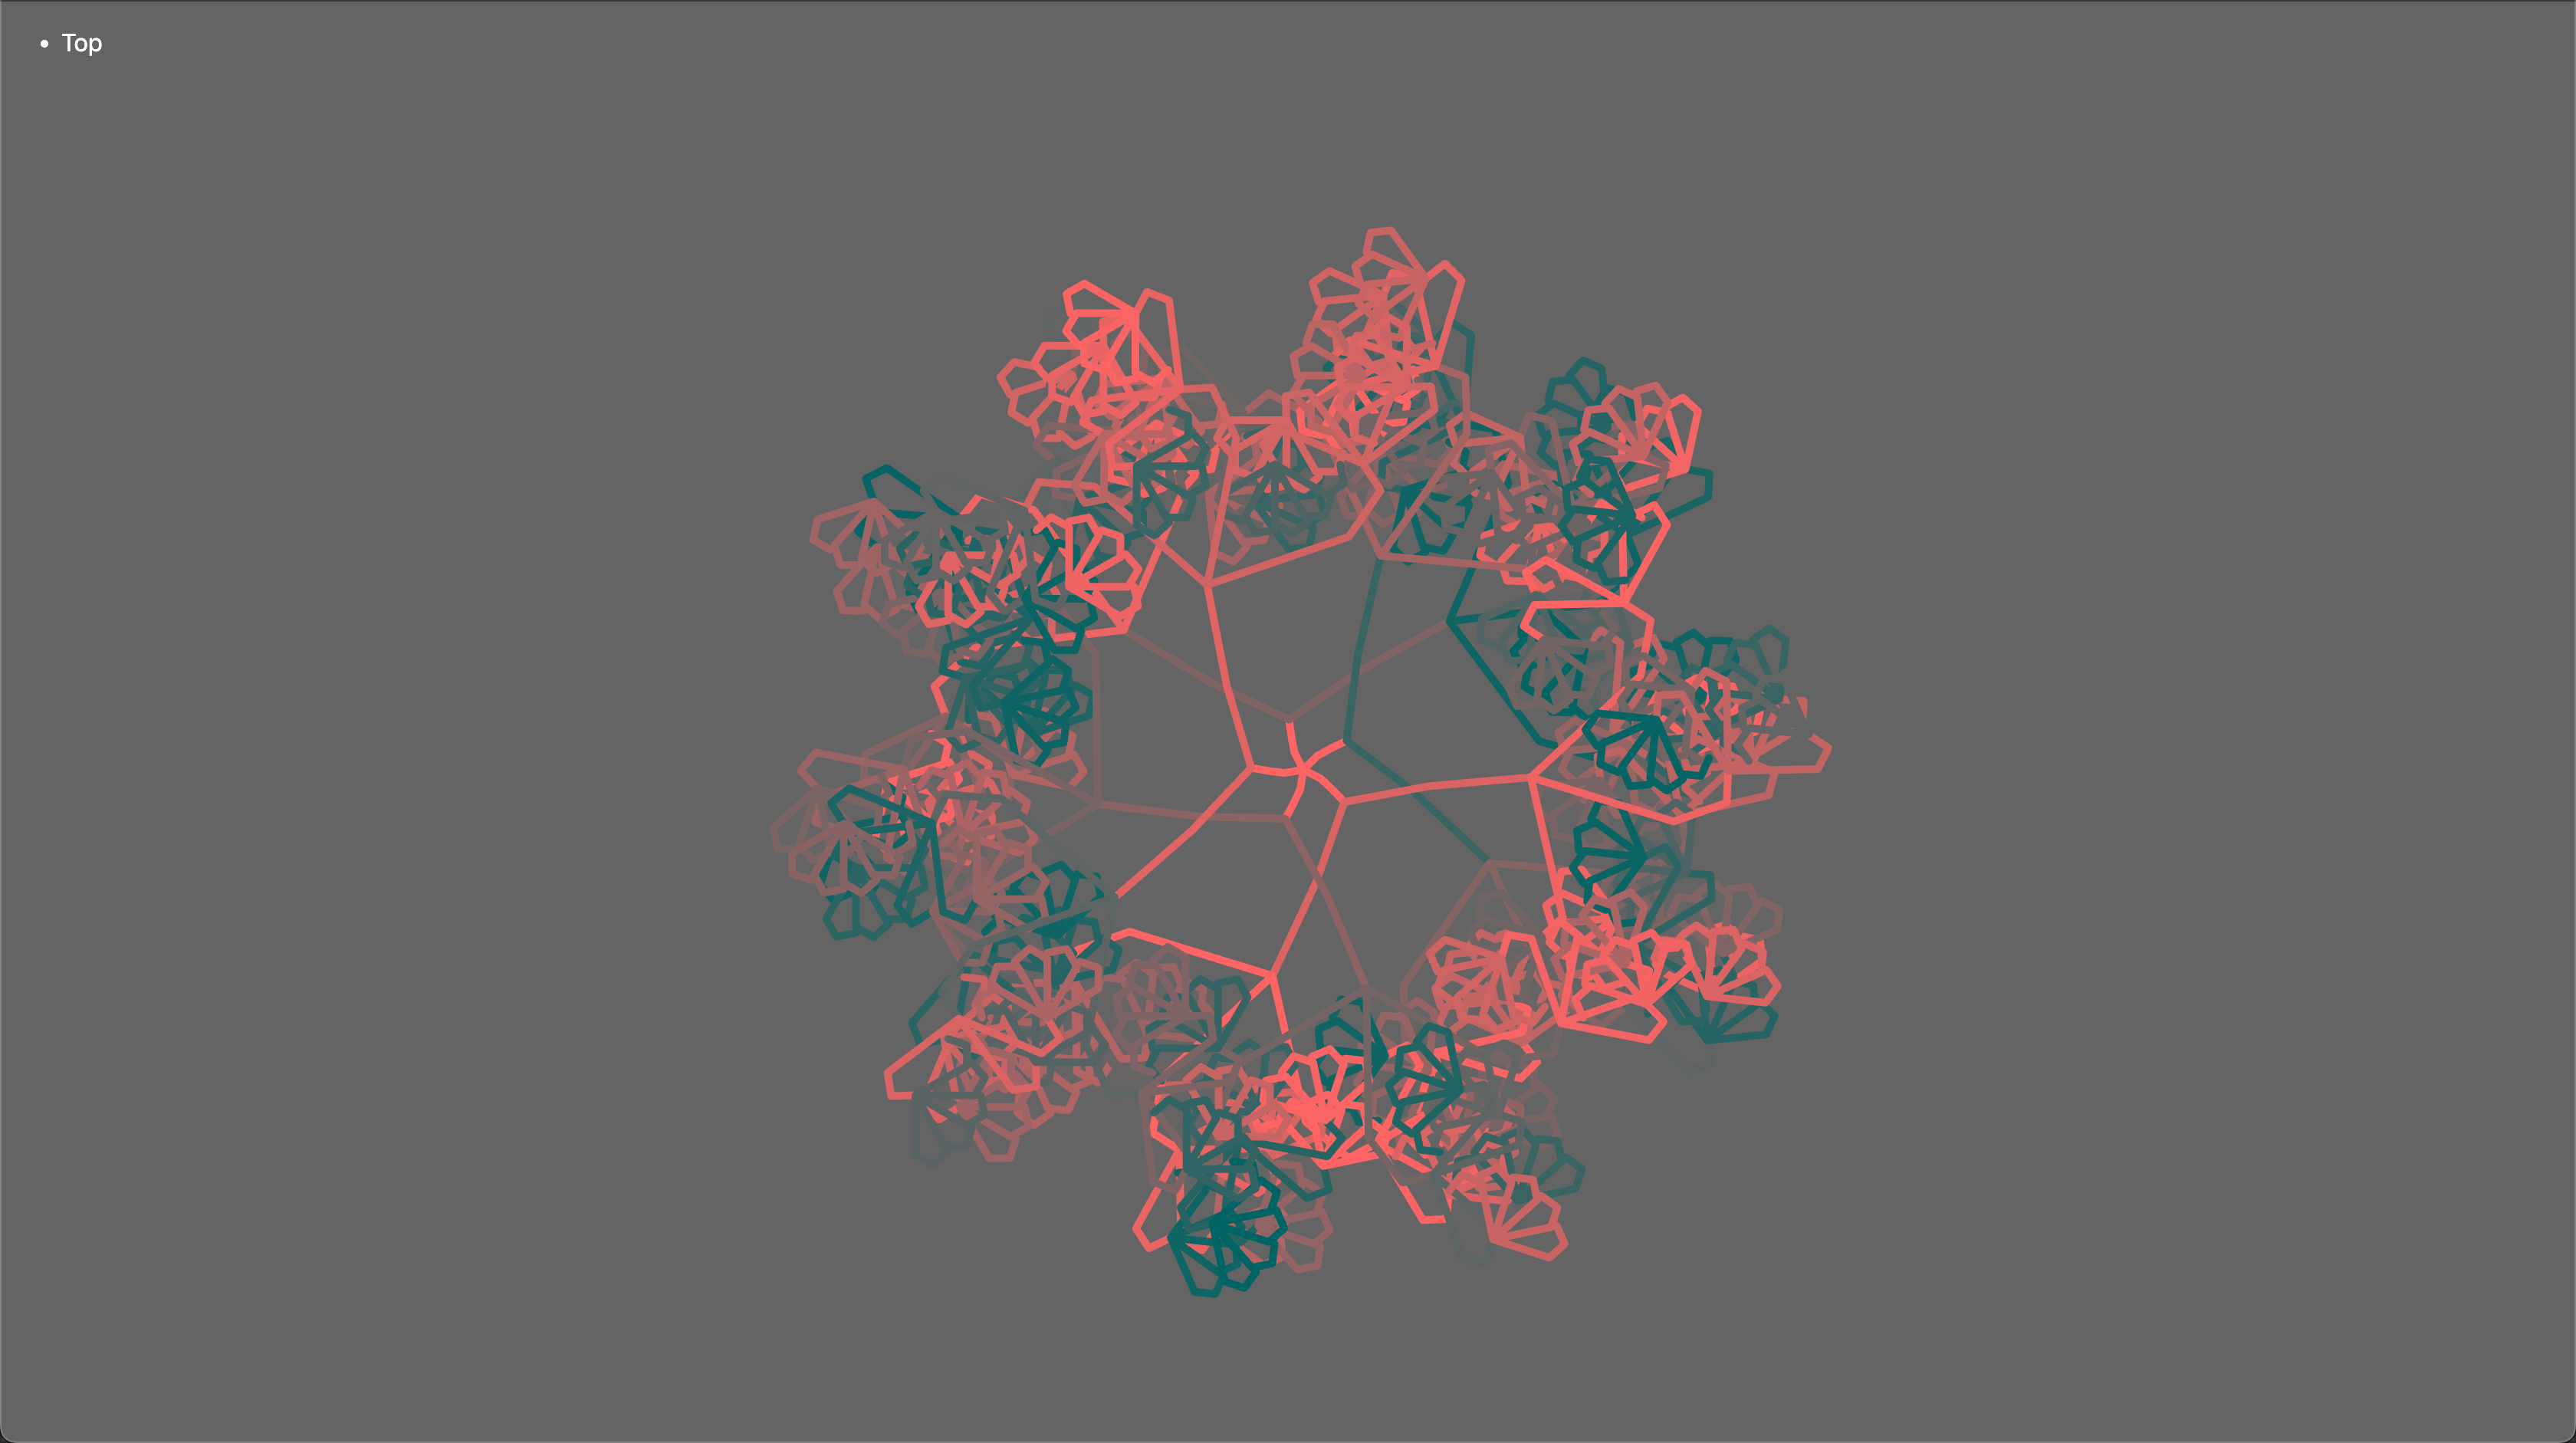
\includegraphics[keepaspectratio, width=7cm]{img/fractel_finger.png}
    \caption{Fractal Finger}
    \label{fig:fractal_finger}
  \end{minipage}
\end{figure}

\subsection{時間操作}
以下は、現在の自分の動きだけを表示するのではなく、過去の動きも表示するバリエーションである。図\ref{fig:prototype_delay}に示すプロトタイプでは、5本の指の動きが等間隔に並べられているが、それぞれの指は、鉛直上向きの角度に現在の指の動き、そこから時計回りに、順次過去の指の動きが並べられている\footnote{\url{https://interaction005-moe5dbh11-k1105.vercel.app/}}。このプロトタイプでは、指先を小さく動かすと、その動きが時計回りに伝播していくような動きが起こる。これは例えばゼリー状の物体を触れた時のような、物体の衝撃が全体へと伝播していくようすにも見立てられる。そのためか、柔らかいオブジェクトに触れているときのような手触りのようなものを感じた。
また、数ミリ秒前の動きが隣接する形に現れ、全体として2秒程の期間の全ての動きが表示されることになる。そのため、2秒間のあいだに動きの変化があれば、身体を動かしていても止まっていても画面に変化が現れることが、直感に反した動きとなることに注意が向く。

\begin{figure}[H]
  \centering
  
\includegraphics[width=15cm]{img/past_time.png}
  \caption{過去の動きを用いた例}
  \label{fig:prototype_delay}
\end{figure}

\subsection{ボール操作}
ここまでは手指をいかに変換するかについて探索を行なってきたが、その手指を用いた動きの複雑度に影響する要素としてボール操作について検討した。こうしたバリエーションを制作し、ボールがないものと並置して「IAMAS openhouse2023」にて展示した際、体験した方の一人から2つを比較して、手指の変換表現だけのものについては「途中から自分が何やってるか忘れてしまって、なんとなく指を動かすとなんとなく画面の描画内容が変わってる、となってしまっている」一方で「ボールの方はそんなことはなかった」とし、その理由として「具体的なタスクがあったほうがずっと続きやすい」といったことを挙げていた。そのため、よりタスクを明確化したバリエーションとして下記のような、マトあてのバリエーションも制作した。

\begin{figure}[H]
  \centering
  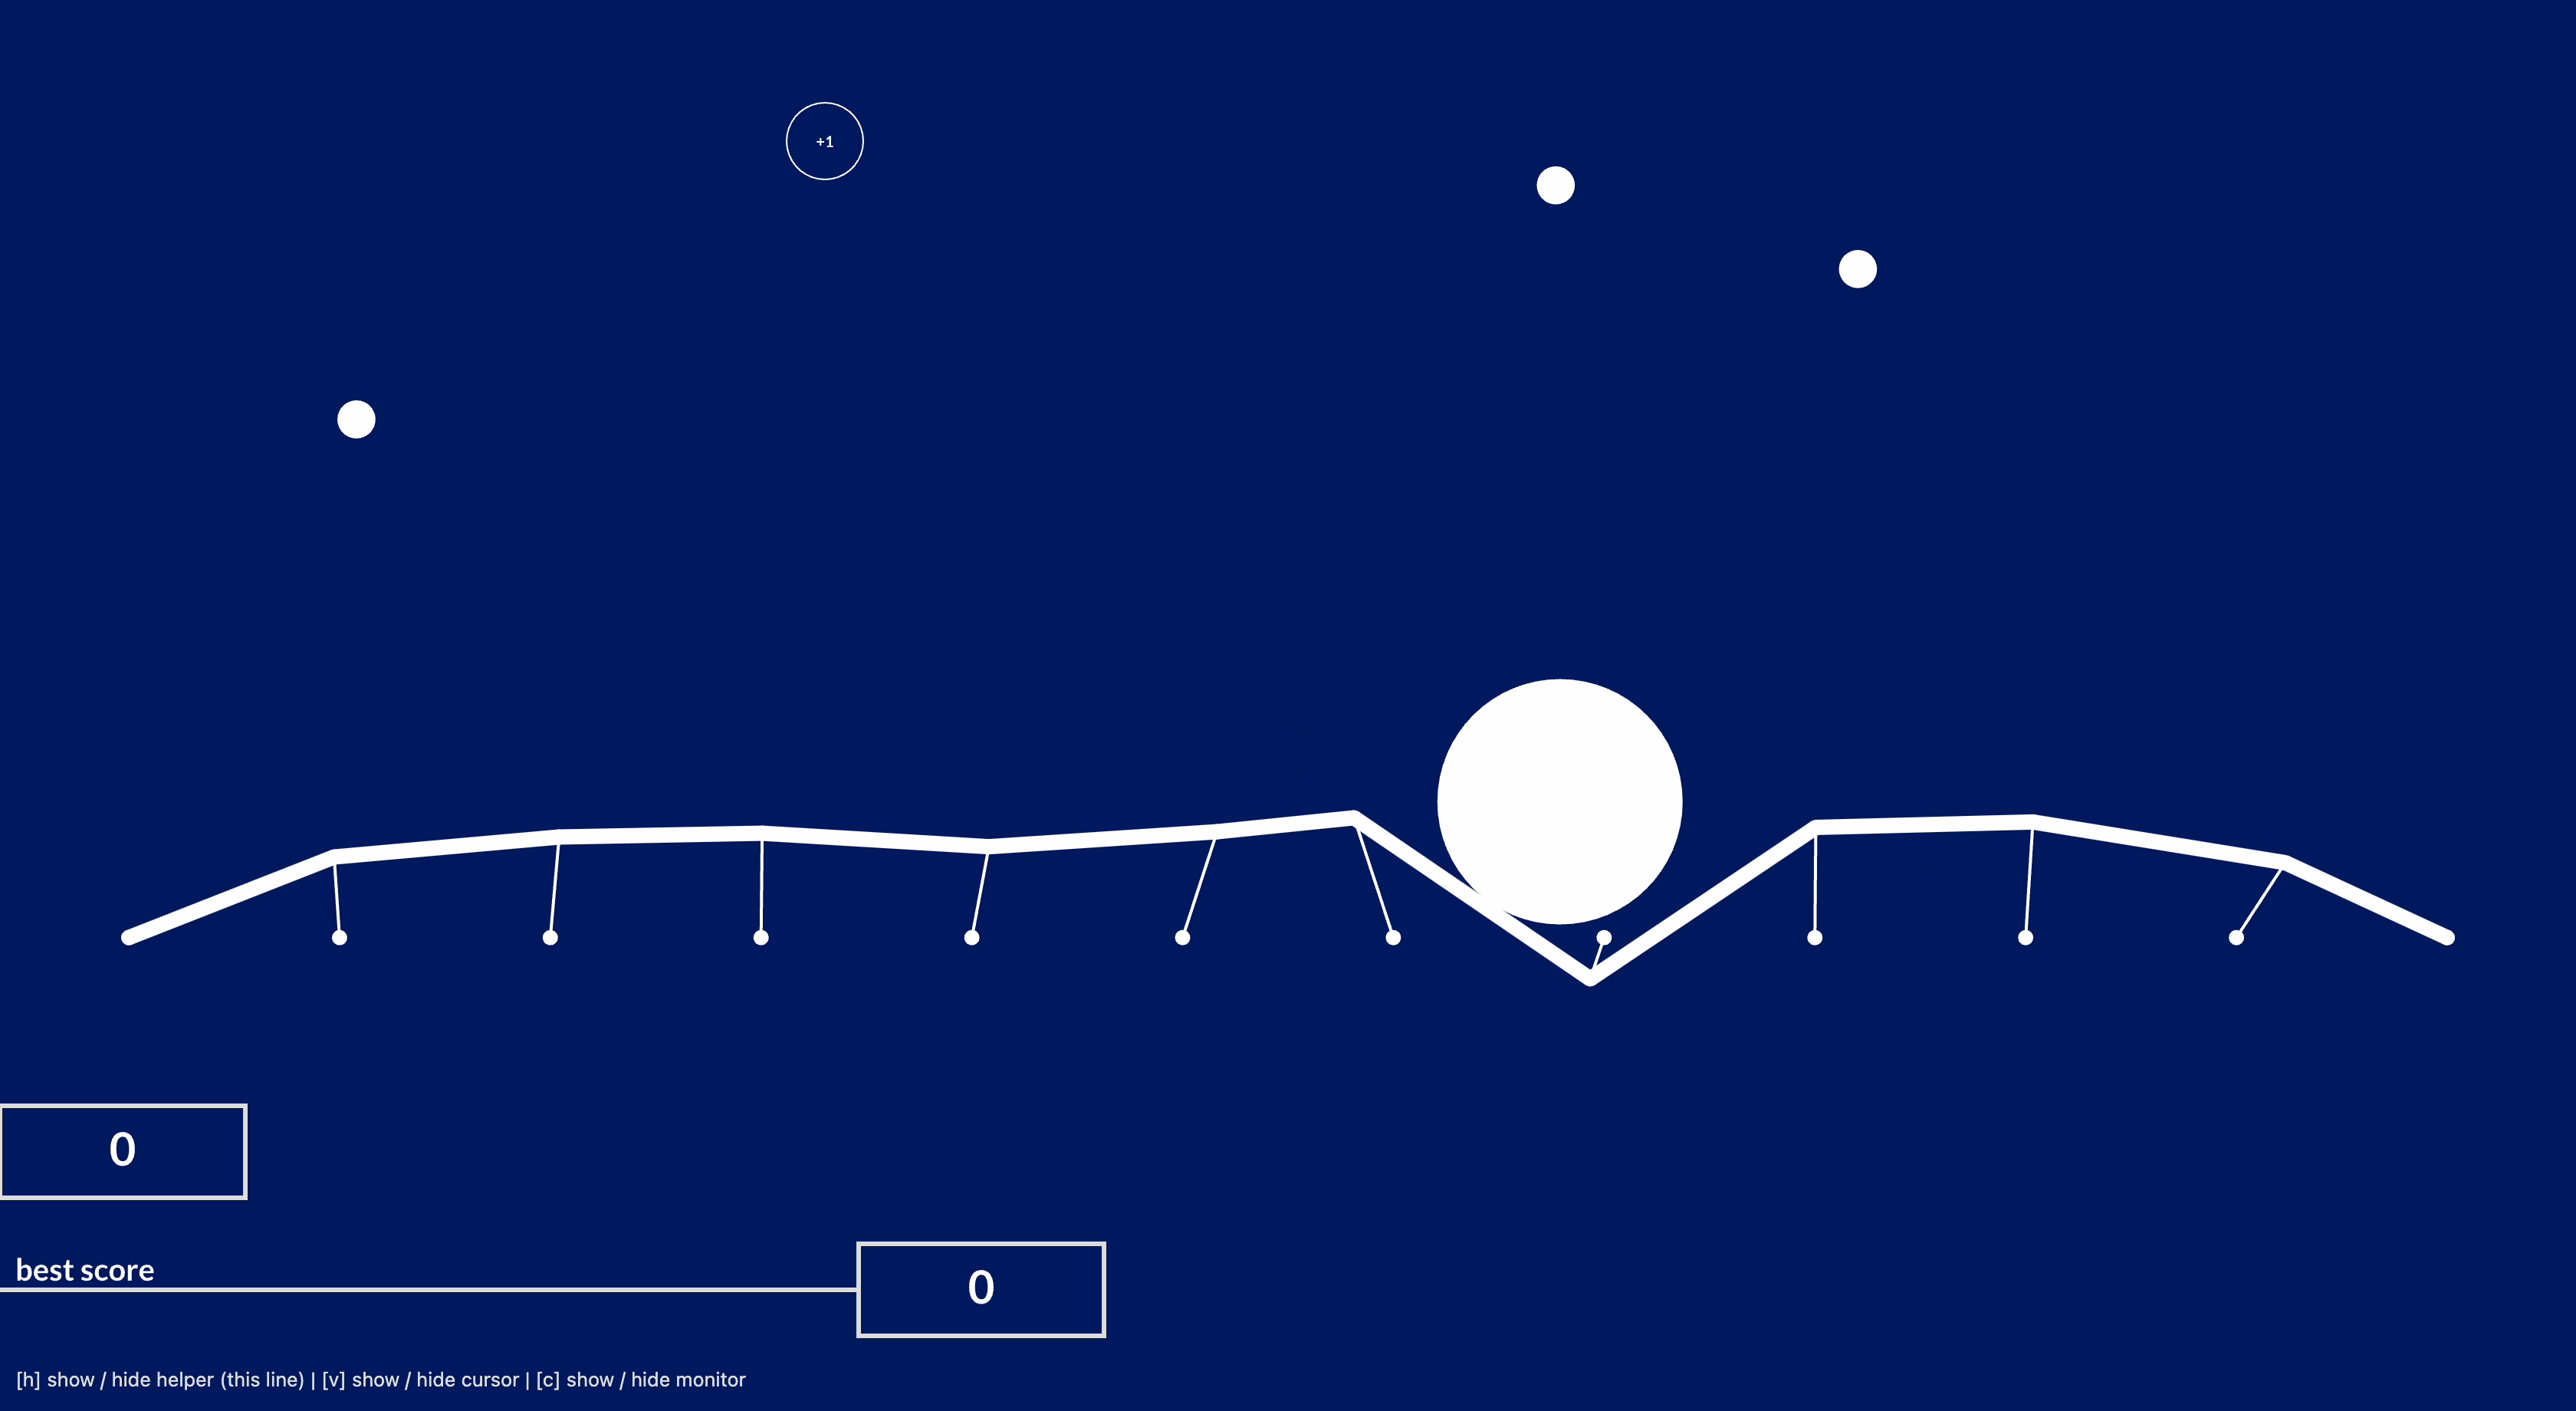
\includegraphics[width=15cm]{img/ball_overview.png}
  \caption{ボール操作の例}
  \label{fig:ball_overview}
\end{figure}

また、過去に制作したバリエーションを拡張する形で、ボール操作のパターンについて検討した\footnote{\url{https://interaction023.vercel.app/}, \url{https://interaction024.vercel.app/}}。

\begin{figure}[htbp]
  \begin{minipage}[b]{0.5\linewidth}
    \centering
    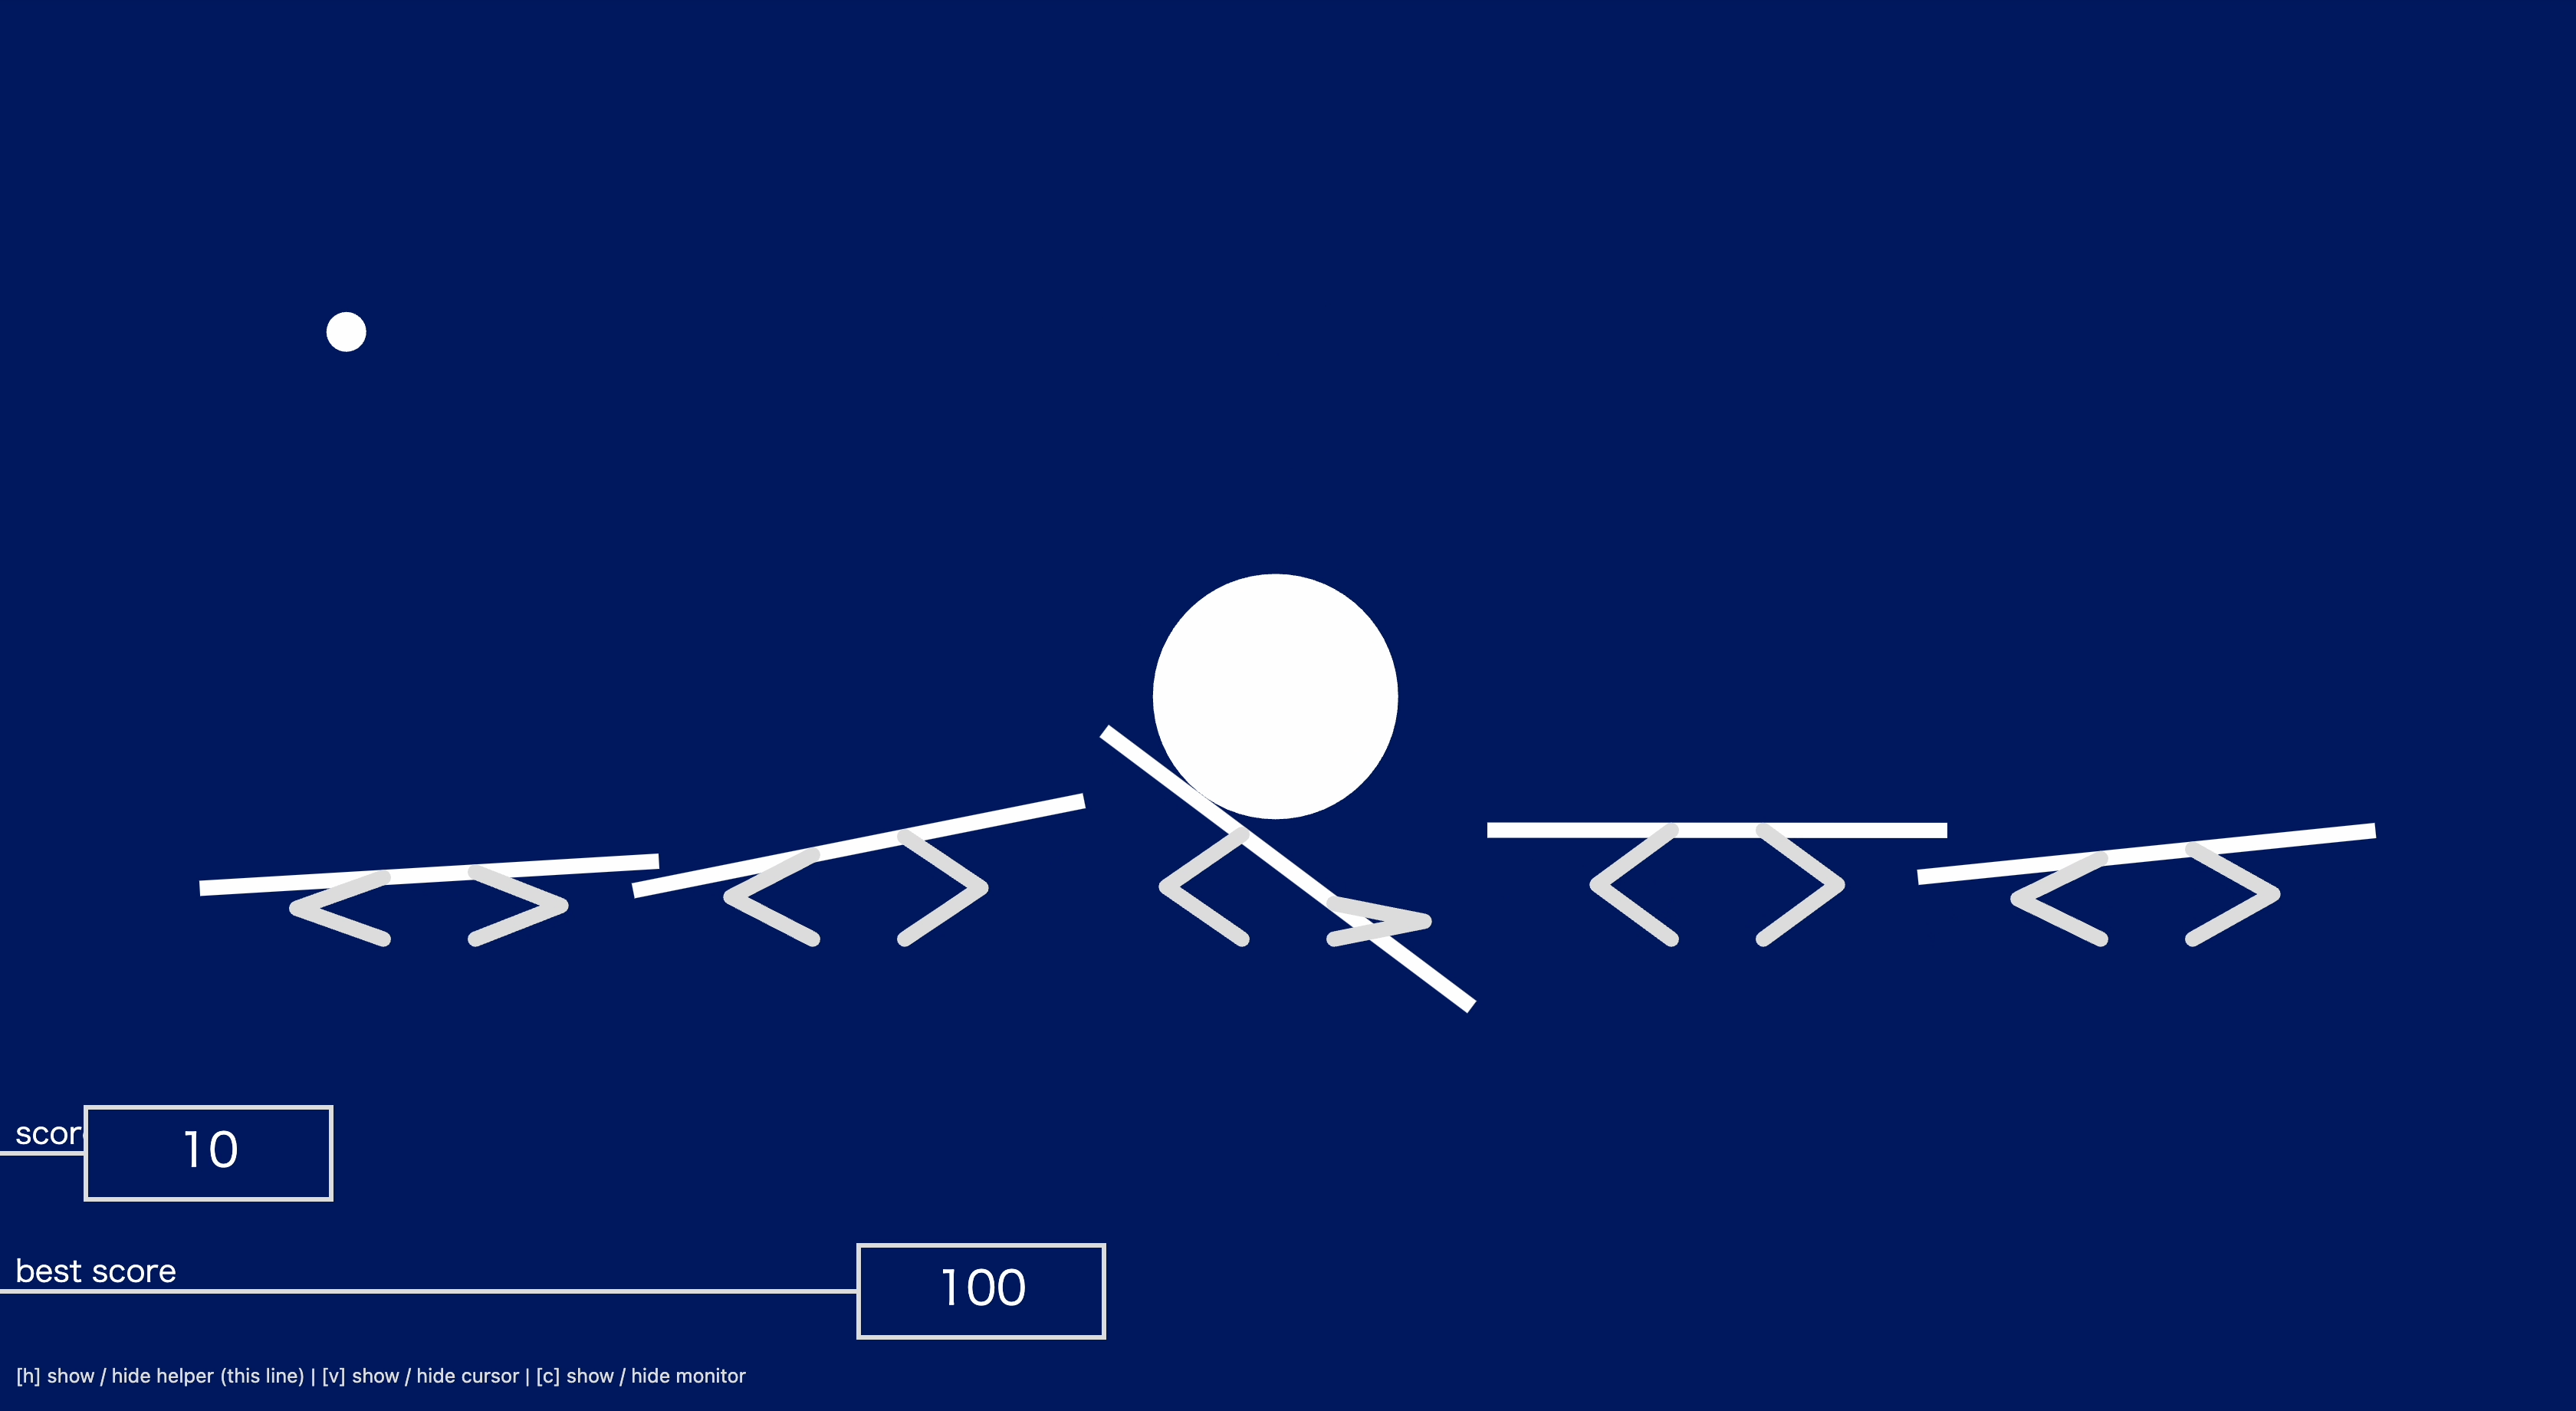
\includegraphics[keepaspectratio, width=7cm]{img/ball_0.png}
    \caption{Networked Finger}
    \label{fig:ball_0}
  \end{minipage}
  \begin{minipage}[b]{0.5\linewidth}
    \centering
    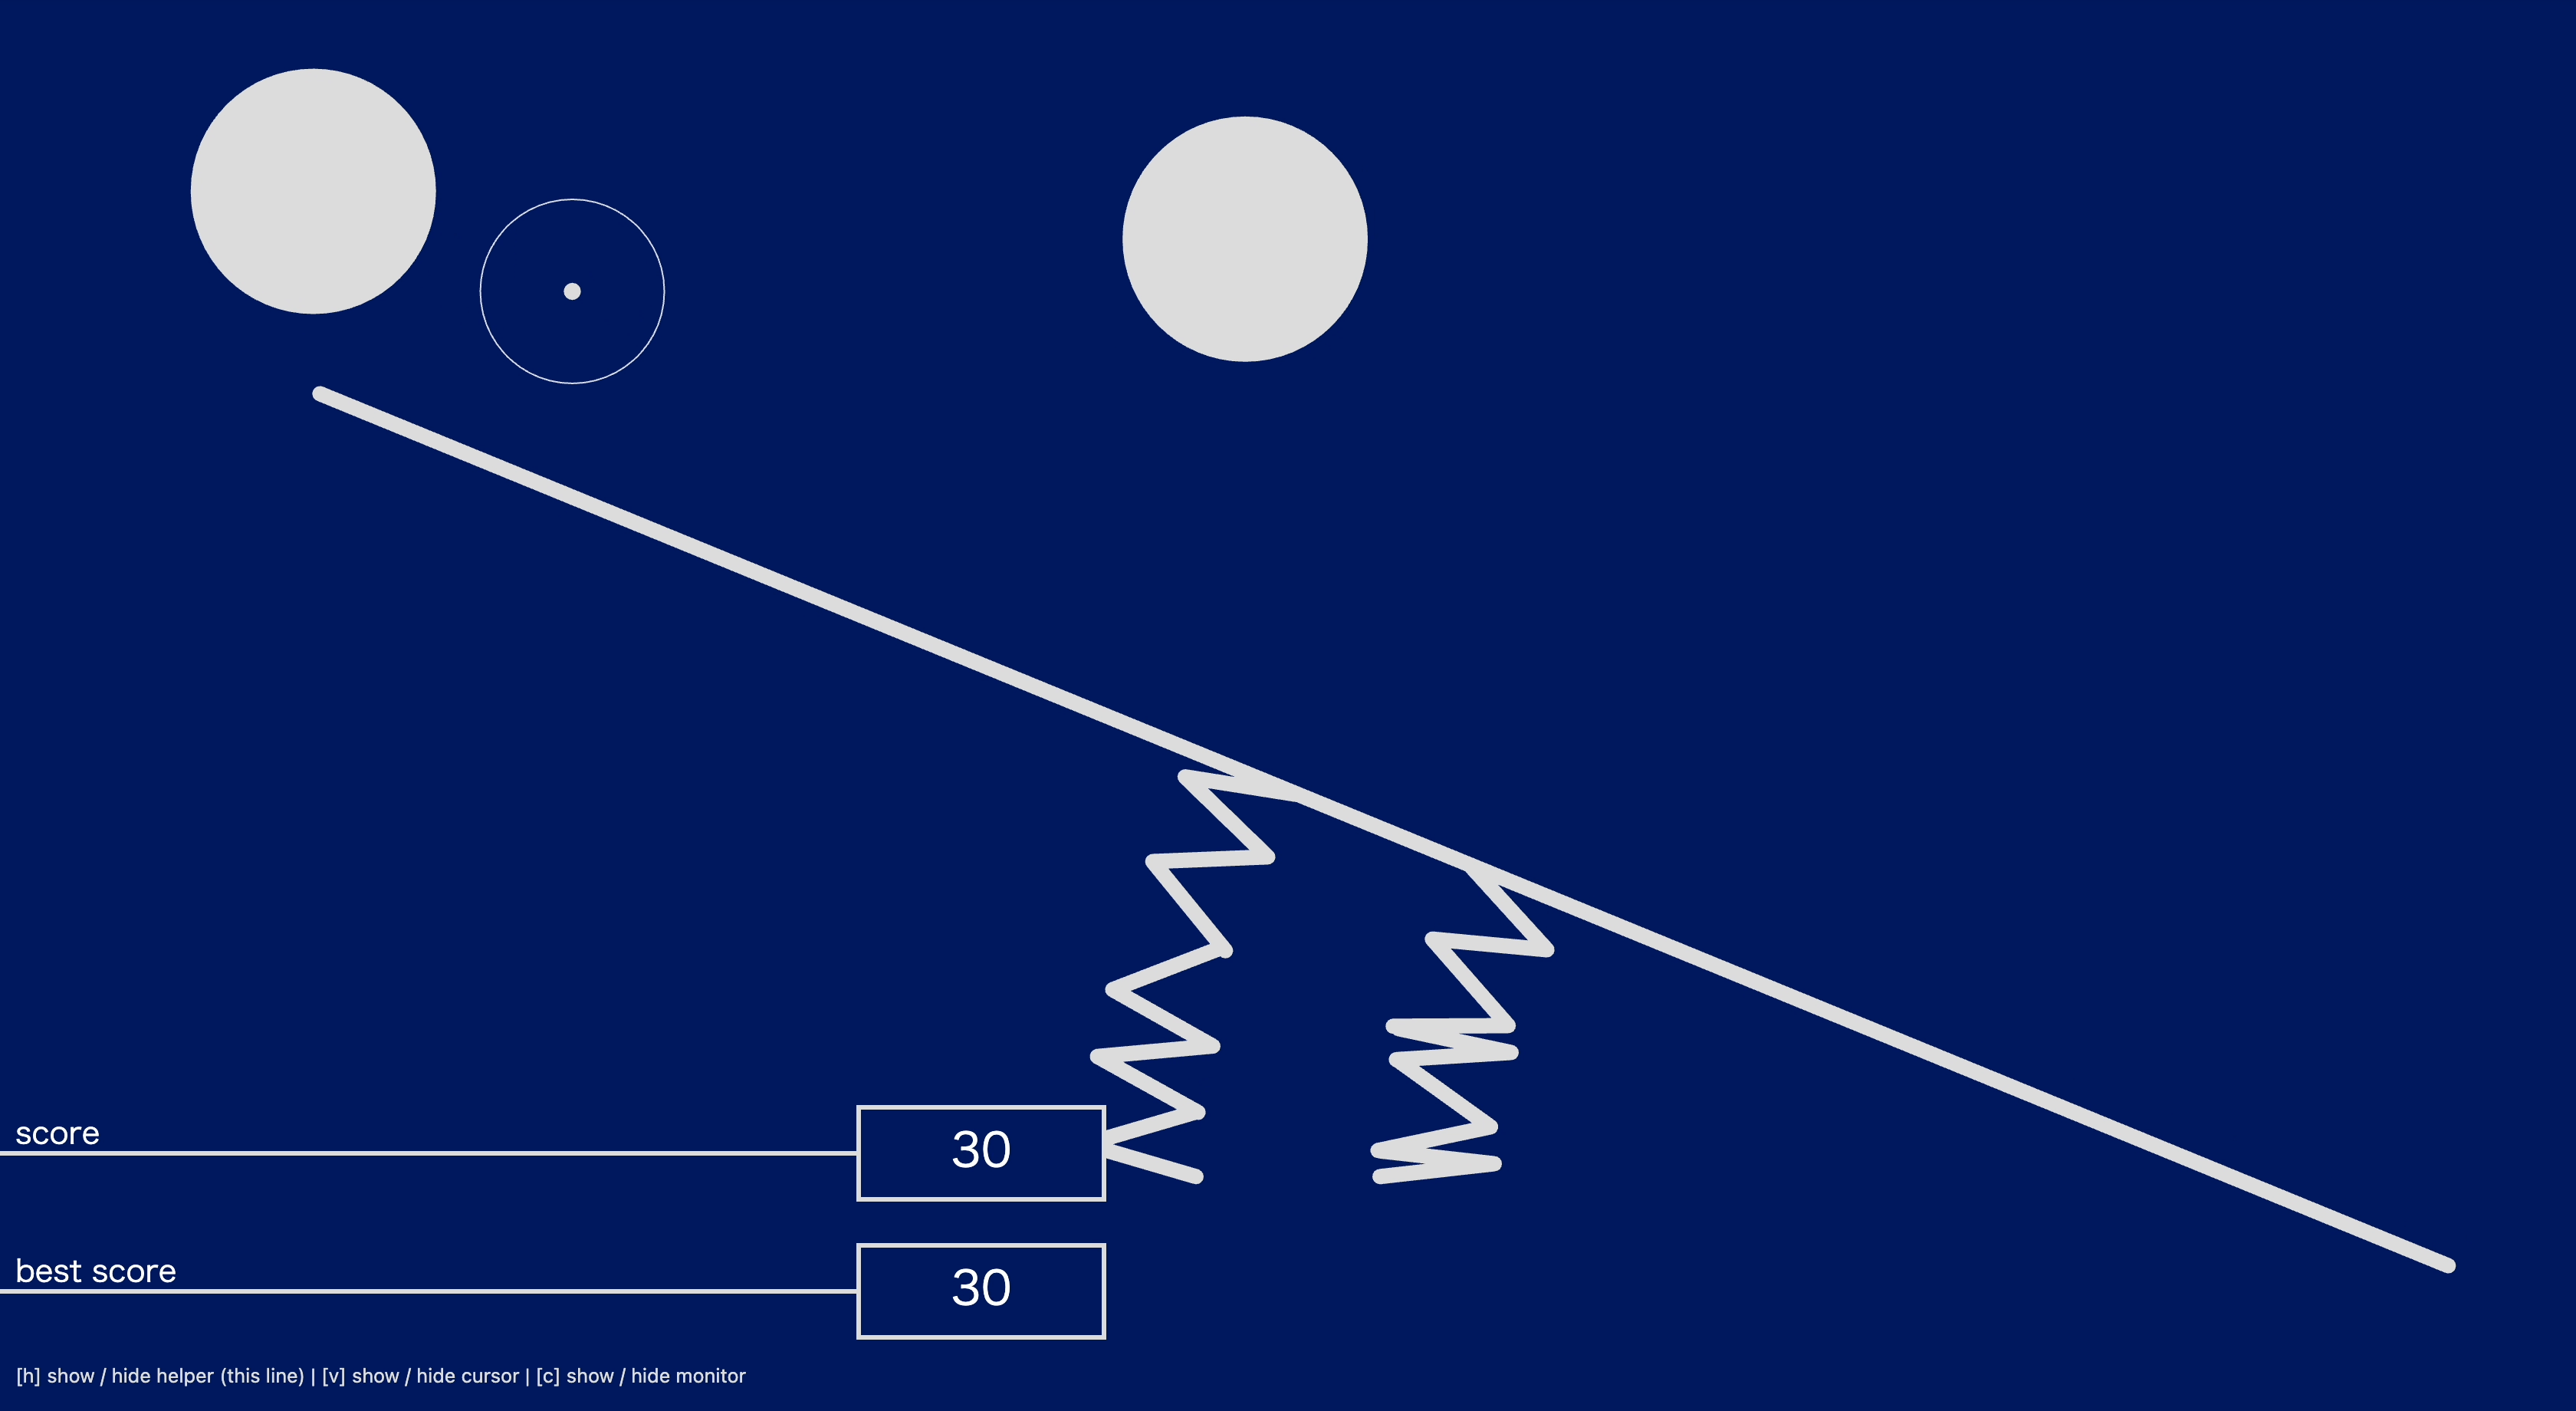
\includegraphics[keepaspectratio, width=7cm]{img/ball_1.png}
    \caption{Fractal Finger}
    \label{fig:ball_1}
  \end{minipage}
\end{figure}

\section{表現の選定}
ここまで、変換表現を扱ったプロトタイプについて概観してきた。以下では、これらのプロトタイプを踏まえて、「人馬一体感」の生起に向け、それを具現化する表現とは何か、という観点から重要だと考えられる観点を列挙し、プロトタイピングについて分析する。

\subsection{動かしている感覚が強い表現}
1つ目の観点として、手指の微細かつ複雑な動きをもって、緻密な制御をしているという感覚が引き出される表現へと絞り込んでいくことにした。

形状については、指を単位としない場合についても検討したが、指は一本一本独立して動かすことができる性質上、指が一つの単位となっている変換に注意を向けやすいのではないかと考えた。その中でも、円形、くの字、ひょうたん型などの変換を試みたが、動きに対して注意が向けられたのは「くの字」の形状であると感じられた。この理由について、身体動作である指の折り曲げとの対応から考察する。

身体動作として指の折り曲げが画面の中で、円の半径へと対応している場合とくの字のような折り曲げ動作に反応している場合とを比べたとき、後者は実際には指先と指の付け根の距離しか評価していないにも関わらず、制御点が3つあるように感じられる。そう捉えると、円の半径が変化していくことよりも対応関係が厳密であり、それを動かすことによって得られる心地よさは、Felsの「Control」による心地よさであると捉えられる。その一方で、円の半径に関節の動きをマッピングさせるような表現については、縮んだり、膨らんだりする動きには共感しづらい。微細な運動が増幅されることに気持ちよさを感じるが、これは身体動作との連動によってもたらされる気持ちよさではなく、動作に対するフィードバックに対する気持ちよさ、すなわちFelsのいう「Response」によるところが強い。

マッピングに関しては、1つの指の動きが規則的に配置される場合について、グラフィックの複雑度が上がっているにも関わらず、感覚としてはより単純な動きであると感じた。これについては、グラフィックデザイナーの女性が体験した際「構造としては緻密であるのに、動きは単純であるように感じる」と意見したことにも重なる。その理由として彼女は、「対称性が前面に出ているため、シンボルとしての印象を強く感じてしまう」「意識していないところも同時に動いている感覚があるため、自分の動きだと思えない」からではないかと推測した。一方で、不規則的に配置される図\ref{fig:networked_finger}のような形状の場合は、1つの動きが複数箇所に複製されているが、指の数が増えると複雑度も比例して上がっているように感じる。これは一つの動きが波及する箇所が多く、動きの予想がつきづらいためではないかと考える。

そのため、1つの動きを複製して円形に配置したり、フラクタル的に配置するパターンは採用しなかった。また、形状についてのバリエーションでの振り返りを通して、関節の動きが身体動作との関連について想起しやすい変換であると考え、それ以外の展開を採用しなかった。

\subsection{注意の対象による作品の分割}
ボール操作に関しては、身体動作を通して直接的に動かすことのできる対象ではないものが現れたことによって、体験の中に「もどかしさ」が生じたと考える。特に、マトのあるときが強かった。これは、明確かつ簡単に達成することのできない目標設定がされることからではないかと考える。また、マトあての利点として、「一体化」の度合いを「いかに器用にマトに当てることができたか」という観点から、客観的にも、主観的にも確かめることができると考えた。しかしその一方で、ボールの出現によって手指だけを動かして感覚を確かめていたときとは、全く異質の体験であると感じた。手指の変換のみが行われていた時には、指一本一本の動きや、それによって構成される全体的な動きに注目していたが、ボールが出現したことによってボールと手の関係性にのみ、注目するようになったと考える。

ボール操作に関するバリエーションを制作した際の気づきから、ボール操作は「もどかしさ」を経験するほどの比較的強い注意を喚起する一方で、ボールがなかった場合と比べると、注意の向く対象が、手指の運動ではなく、ボールと手指の関係性に注意が生じることがわかった。そこで、最終的な作品としてはその2つを分けて構成した。そして、手指の形状が変化することを起点に注意が生じる作品と、ボールと手指との関係性に注意が生じる作品というように、何に注意が生じるかという観点に着目して2つの体験を整理した。

また、ボールの現れる作品においては、プロトタイピングの過程で表示していた「スコア」を設けなかった。理由として、スコアが存在することで「マトに当てる」という目的意識を強く与えてしまうことが挙げられる。強固な目的意識の設計は、より多くの人を同一の目的に向かわせ、一定の体験が期待できる一方で、その目的以外の興味や注意が生じる余地を排斥してしまうと考えた。

\subsection{モーフィングの追加}
過去に展示していたバージョンではモーフィングを示さず、手指が認識されたとたんに全く違う手指が提示される作品形態であった。しかし、この形態で展示した場合、画面の中の手指と自身の関係性について意図しない受け取られ方をすることに気づいた。つまり、全く異なる生命体のようなものを、操り人形のように自分の手指の指令によって動かす、といったような関係性として認識されることがある。また、全く見慣れない形なので「手指を細かく動かせる」といった、作品がもつ可能性に気づけないことがある。そこで、形状の変化を確認できるモーフィングを実装した。そうすることで、白い点が関節を表していること、そして手指の運動を細かくトラッキングしていることを事前に伝え、それが形を変えた姿として画面の前に提示されていることがわかるようになる。

\section{展示形態の設計}
展示形態について、時系列順に過去2つのバージョンについて説明し、その流れから最終的な展示形態の根拠を示す。

\textbf{初期:カメラを画面前に配置した状態}\\
最初期は、体験装置について下図\ref{fig:kyotai_ver0}のように、モデルトラッキングを行っているカメラを直接画面の前に配置していた。
\begin{figure}[H]
  \centering
  \includegraphics[width=12cm]{img/kyotai_ver0.jpg}
  \caption{初期:カメラを画面前に配置した状態}
  \label{fig:kyotai_ver0}
\end{figure}

プロトタイピングの段階でもあったため最低限の構成としていたが、この構成には次のような問題があった。
\begin{quote}
  \begin{itemize}
    \item カメラのトラッキング精度が環境光の影響を受けて変動してしまう
    \item 体験者ではない周囲の人の手指を間違ってトラッキングしてしまう
    \item 手指の形がそのまま出力されるわけではないので、トラッキングの範囲がわからず、腕を大きく振ったり、手指がトラッキングできない範囲で動かしてしまう
  \end{itemize}
\end{quote}

このため、制作者が指示をすることなく自由に体験してもらうことを意図していた展示であっても、体験方法がわからなかったり、後方で見守る人の手を誤ってトラッキングしてしまうといった問題が起き、有効なフィードバックを得ることができなかった。

\textbf{中期:専用筐体を用いて手首を固定した状態}\\
こうした課題を踏まえて、次に専用筐体を制作し、穴に手を入れる形式について試した(図\ref{fig:kyotai_ver1})。

\begin{figure}[H]
  \centering
  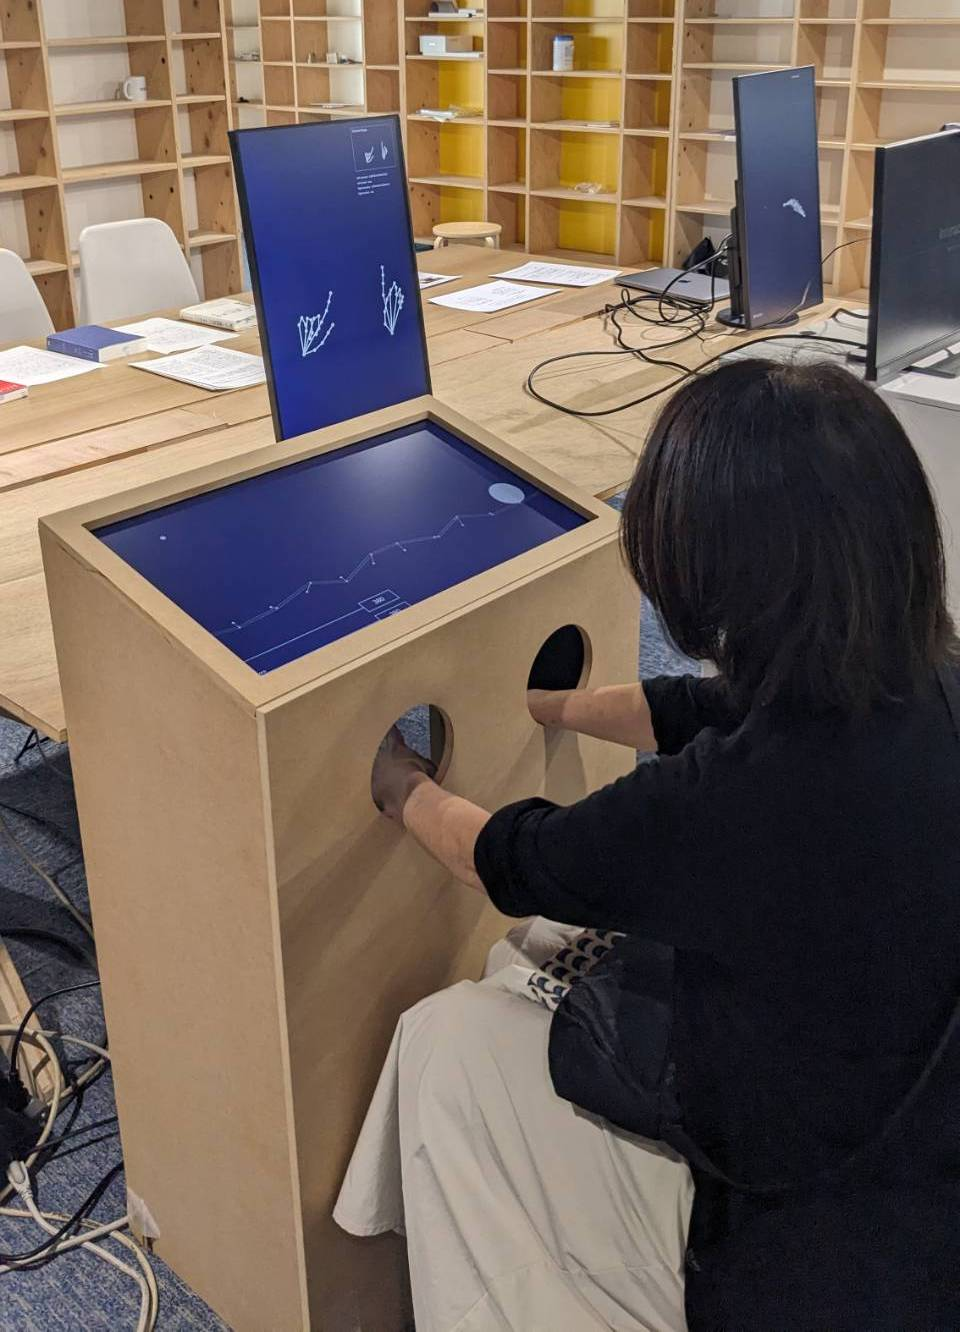
\includegraphics[width=8cm]{img/kyotai_ver1.jpg}
  \caption{中期:専用筐体を使用してカメラを隠蔽した状態}
  \label{fig:kyotai_ver1}
\end{figure}

この形式では、カメラの画角に映り込むのは筐体の内部と体験者の手のみであるため、環境光の影響や周囲の人の影響を受けずに体験できるようになった。また、穴によって手首の位置が固定されるため、腕を大きく振ることが構造上不可能となり、比較的身体動作の幅が抑えられた。

ただし、この形式は単に上記の問題を解決したというだけではなく、指先の動きが見えなくなったこと、画面に対する指先の位置関係についてを変更するものであった。

画面に対する手指の位置関係については、本作品では手指の形状が、もとの形とは全く関係のない構造へと変化するため、作品体験には大きな影響はないと判断した。手指の動きが見えなくなったことについては、画面の中の手指は体験時、自身の身体に代わる存在であるから、同時に視認できない今の形態の方がむしろ、より適した構成であると判断した。

しかしその一方で、手首の動きを固定してしまったことは、身体の動きを過剰に限定してしまう結果となった。身体の動きを限定してしまうと、何か特定の動作を求められているような説明的な構成になってしまう。そのため筐体としては、より簡素な構成が好ましいと判断した。


\textbf{作品展示:専用筐体を用いて手首を固定せず指先を自由にした状態}\\
そこで最終的には、図\ref{fig:kyotai_ver2}のような、トラッキングの範囲を暗示しながら、手首を固定しない方式に変更した。また、トラッキングに用いるカメラを、視野角150°の広角カメラ(Sanwa Supply CMS-V43BK-3)に変更し、大きく手指を動かしてもトラッキングの外れることの少ないものへと変更した。

\begin{figure}[H]
  \centering
  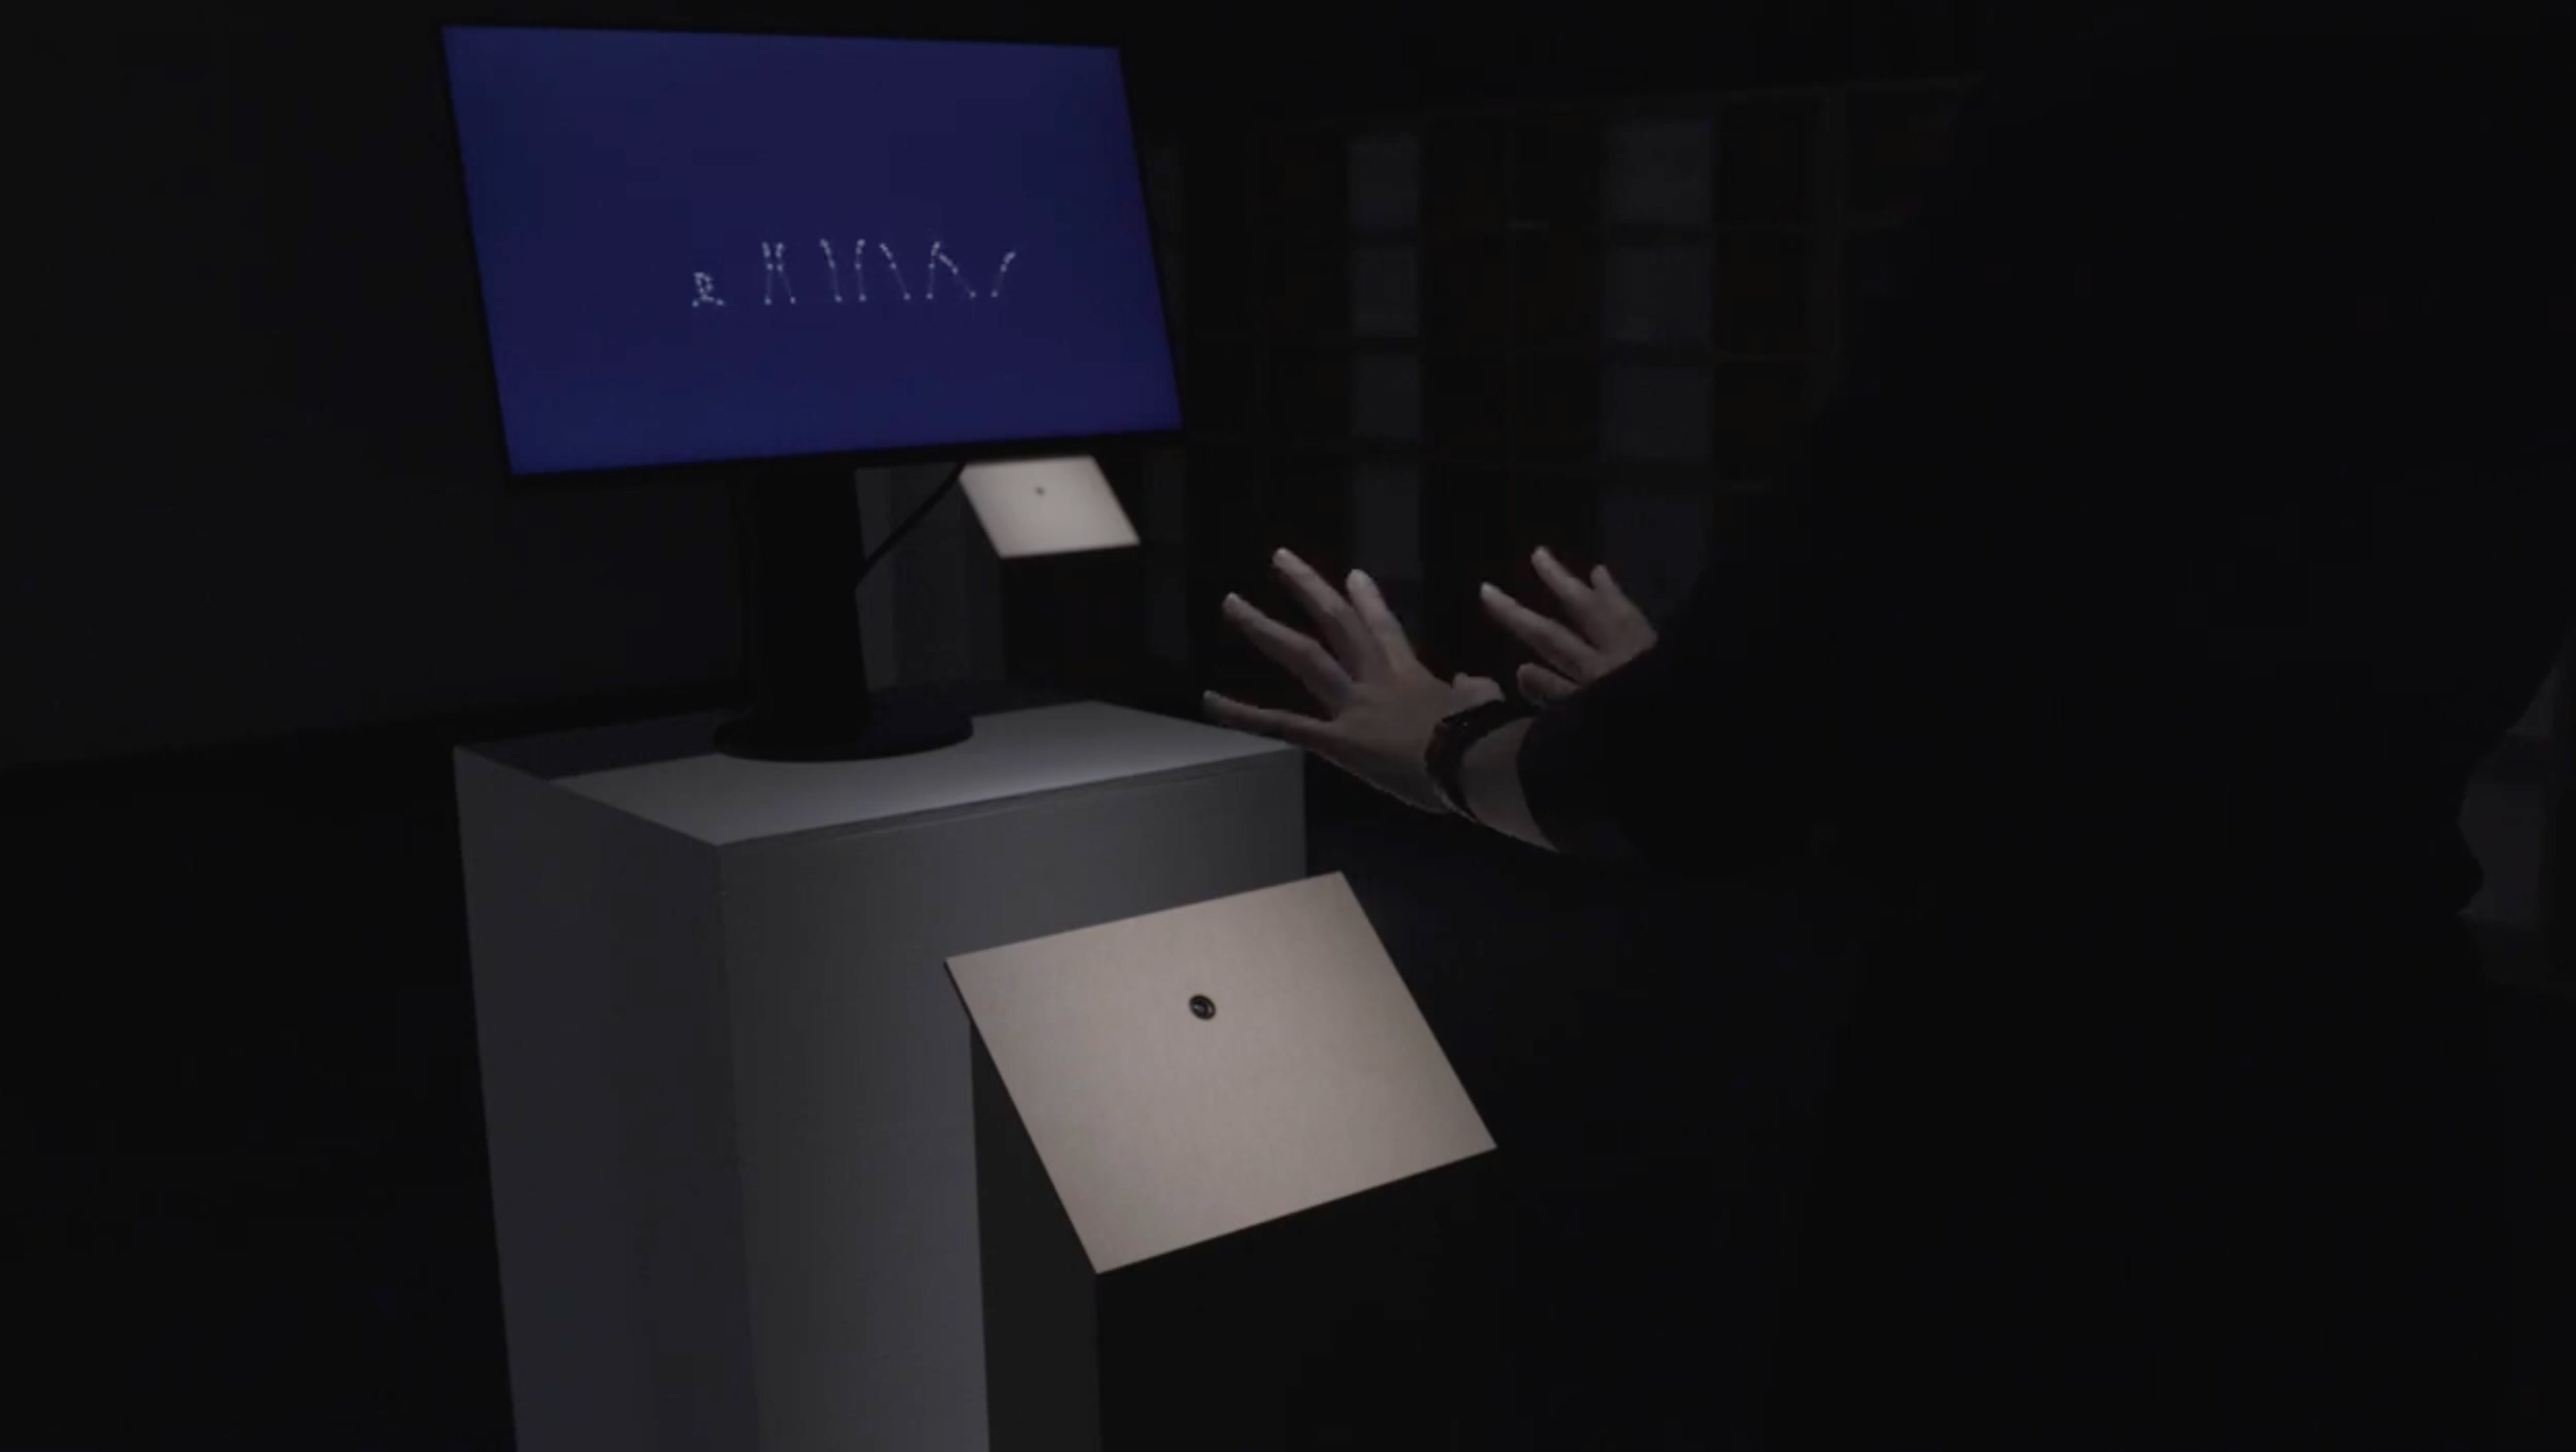
\includegraphics[width=12cm]{img/kyotai_ver2.png}
  \caption{作品展示の際の筐体}
  \label{fig:kyotai_ver2}
\end{figure}

筐体の高さは腰ほどの高さ(850mm)とすることで、キーボードのブラインドタッチのように、画面を見ながら手を同時に見ることが難しい構成とした。

カメラは、鉛直上向ではなく斜めを向いているので、筐体の前に立つと体験者の身体と手指の位置が重なり、トラッキングしやすい状況ができる。

また、ライティングの調整によってトラッキングの精度を高めた。
最終的な展示形態では、スポットライトを当てることで筐体周りを明るくすると同時に照り返しで手元の採光をし、周囲の照明を落とすことで明暗差を作ることで、手指の姿勢を認識しやすくなる。

\begin{figure}[H]
  \centering
  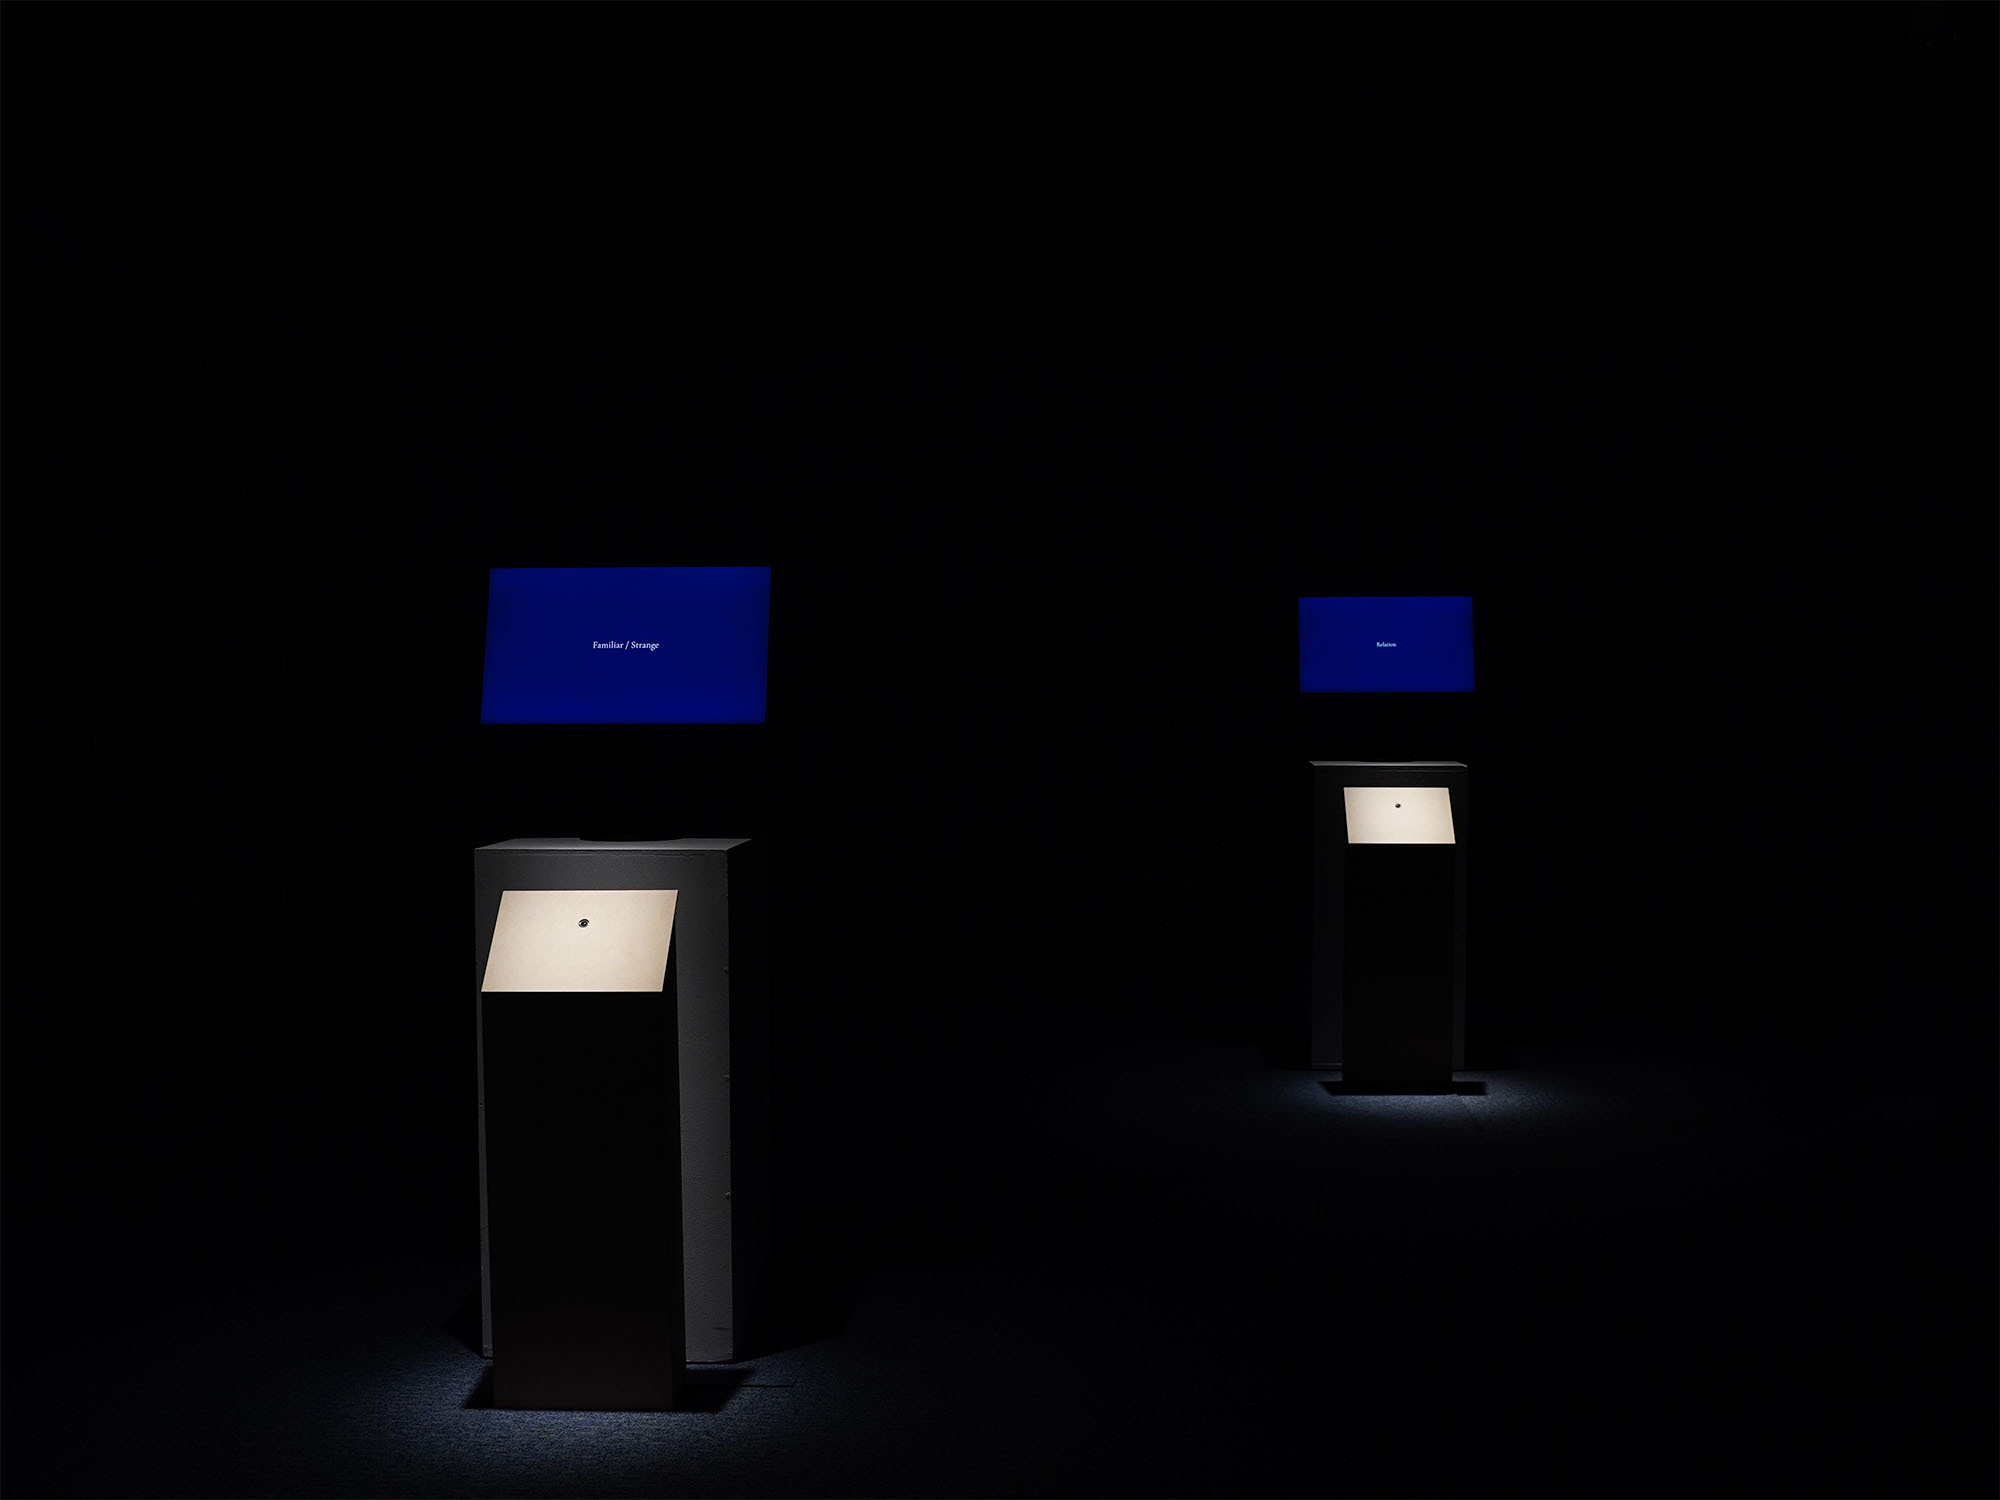
\includegraphics[width=12cm]{img/lighting.jpg}
  \caption{作品展示の際のライティング}
  \label{fig:lighting}
\end{figure}

\section{ライブラリの開発}
本作品を構成するにあたり、基本的な関数をまとめたライブラリを開発した。ライブラリには、円滑に体験するための補完処理を実装している。
具体的には、ガウシアンフィルターによる平滑化処理、トラッキングが途切れた際の例外処理の2つである。

\subsection{ガウシアンフィルターによる平滑化処理}
推定精度の問題から、モデルより推定される姿勢情報をそのまま出力すると、手指を動かしていなくても小刻みに振動したり、一時的なフレームレートの低下に起因してスムーズに動作していないように感じることがある。\\
そこで、体験者にフィードバックする際に使用する姿勢情報は、前後2フレーム分のフレーム情報にガウシアンフィルターを適用した平滑化処理を実装している。ただし、トラッキングが開始した直後は5フレーム分のフレーム情報を使用することができないため、この場合は取得できる限りのフレーム情報を用いて同じ処理を行なっている。
% そのため以下では、各フレーム情報に対する重みづけと、それを用いて体験者に提示される姿勢情報を求める上での一般式を示す。
% モデルより推定された最新の姿勢情報を\(P_{n}\)、出力されている姿勢情報を\(S\)とすると、
%   % 平滑化フレーム S の定義
%   \begin{equation}
%     S = \sum_{i=-2}^{2} w_i' \cdot P_{n+i}
%     \end{equation}

% ここで、\(w_i'\)は正規化されたガウシアンフィルタの重みを表す。正規化前の重み\(w_i\)は、
% \begin{equation}
%   w_i = \frac{1}{\sqrt{2\pi}\sigma} e^{-\frac{i^2}{2\sigma^2}}
%   \end{equation}

% 正規化された重み\(w_i'\)は、
%   % 重みの正規化
%   \begin{equation}
%   w_i' = \frac{w_i}{\sum_{j=-2}^{2} w_j}
%   \end{equation}
% と表現される。
この処理のため、最良時で60fps程度で取得される姿勢情報は、慢性的に0.3sほどの遅延を伴って体験者にフィードバックされることになる。

\subsection{トラッキングが途切れた際の例外処理}
体験時、環境光や、手指を動かす範囲や速度の関係から、トラッキングが途切れることがある。素早い動きをしている最中に1フレームでも途切れると円滑に体験することができないため、この時は例外的に、トラッキングが途切れる直前のフレーム情報で失われたフレーム情報を埋め合わせる処理を実装した。また、トラッキングが途切れていることに起因する不快感は、本作品の体験外の問題なので、手指の動きがトラッキングできていない状態を視覚的にフィードバックするため、トラッキング不能時に塗りつぶしを透過する視覚効果を実装した(\ref{fig:track_true}, \ref{fig:track_false})。

\begin{figure}[htbp]
  \begin{minipage}[b]{0.5\linewidth}
    \centering
    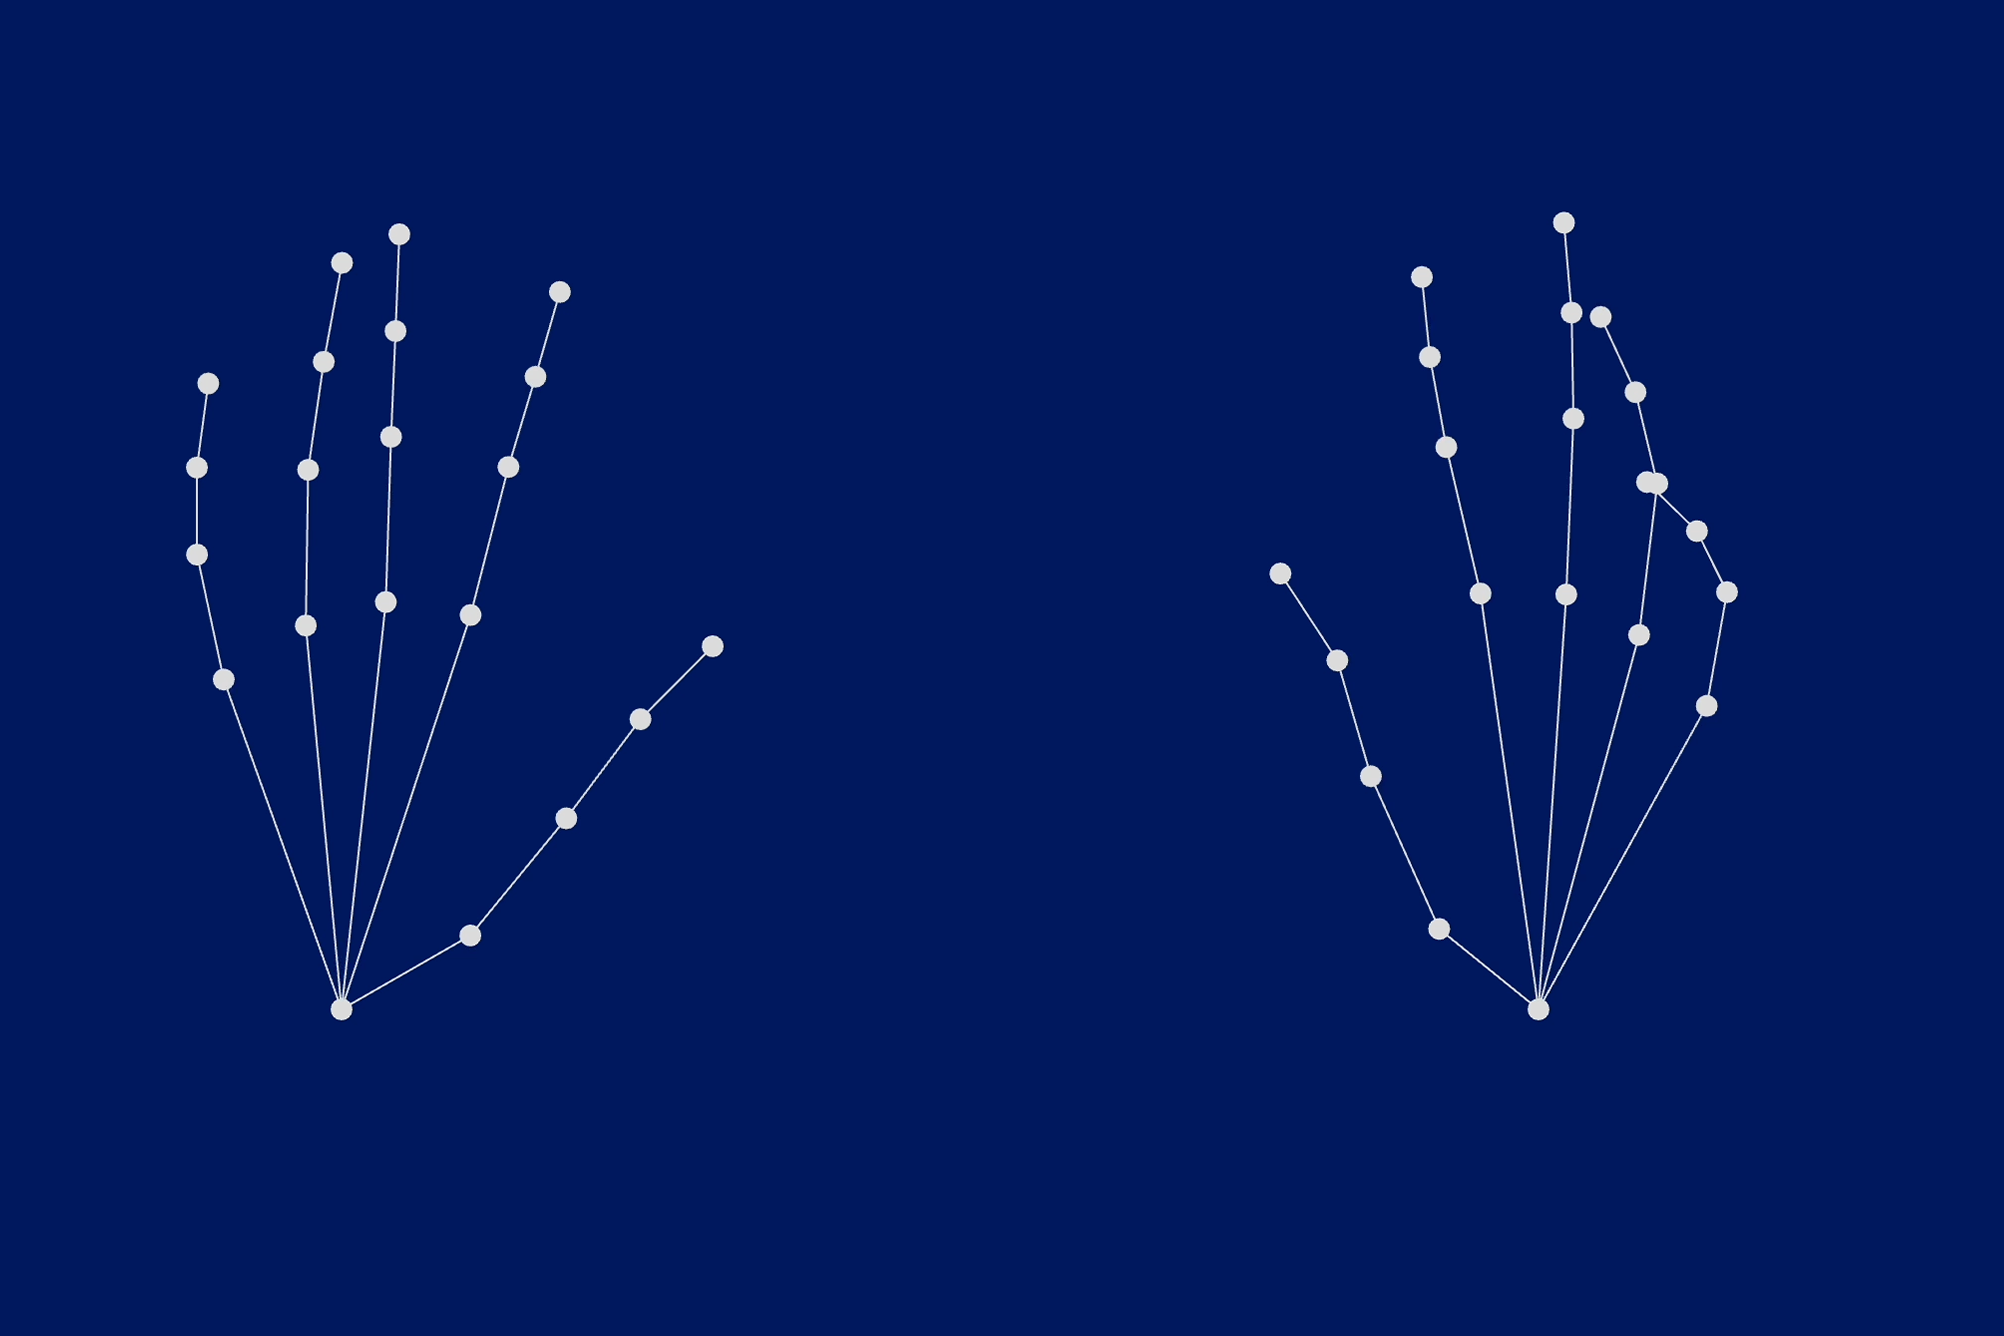
\includegraphics[keepaspectratio, width=7cm]{img/track_true.png}
    \caption{トラッキングが正常にできているとき}
    \label{fig:track_true}
  \end{minipage}
  \begin{minipage}[b]{0.5\linewidth}
    \centering
    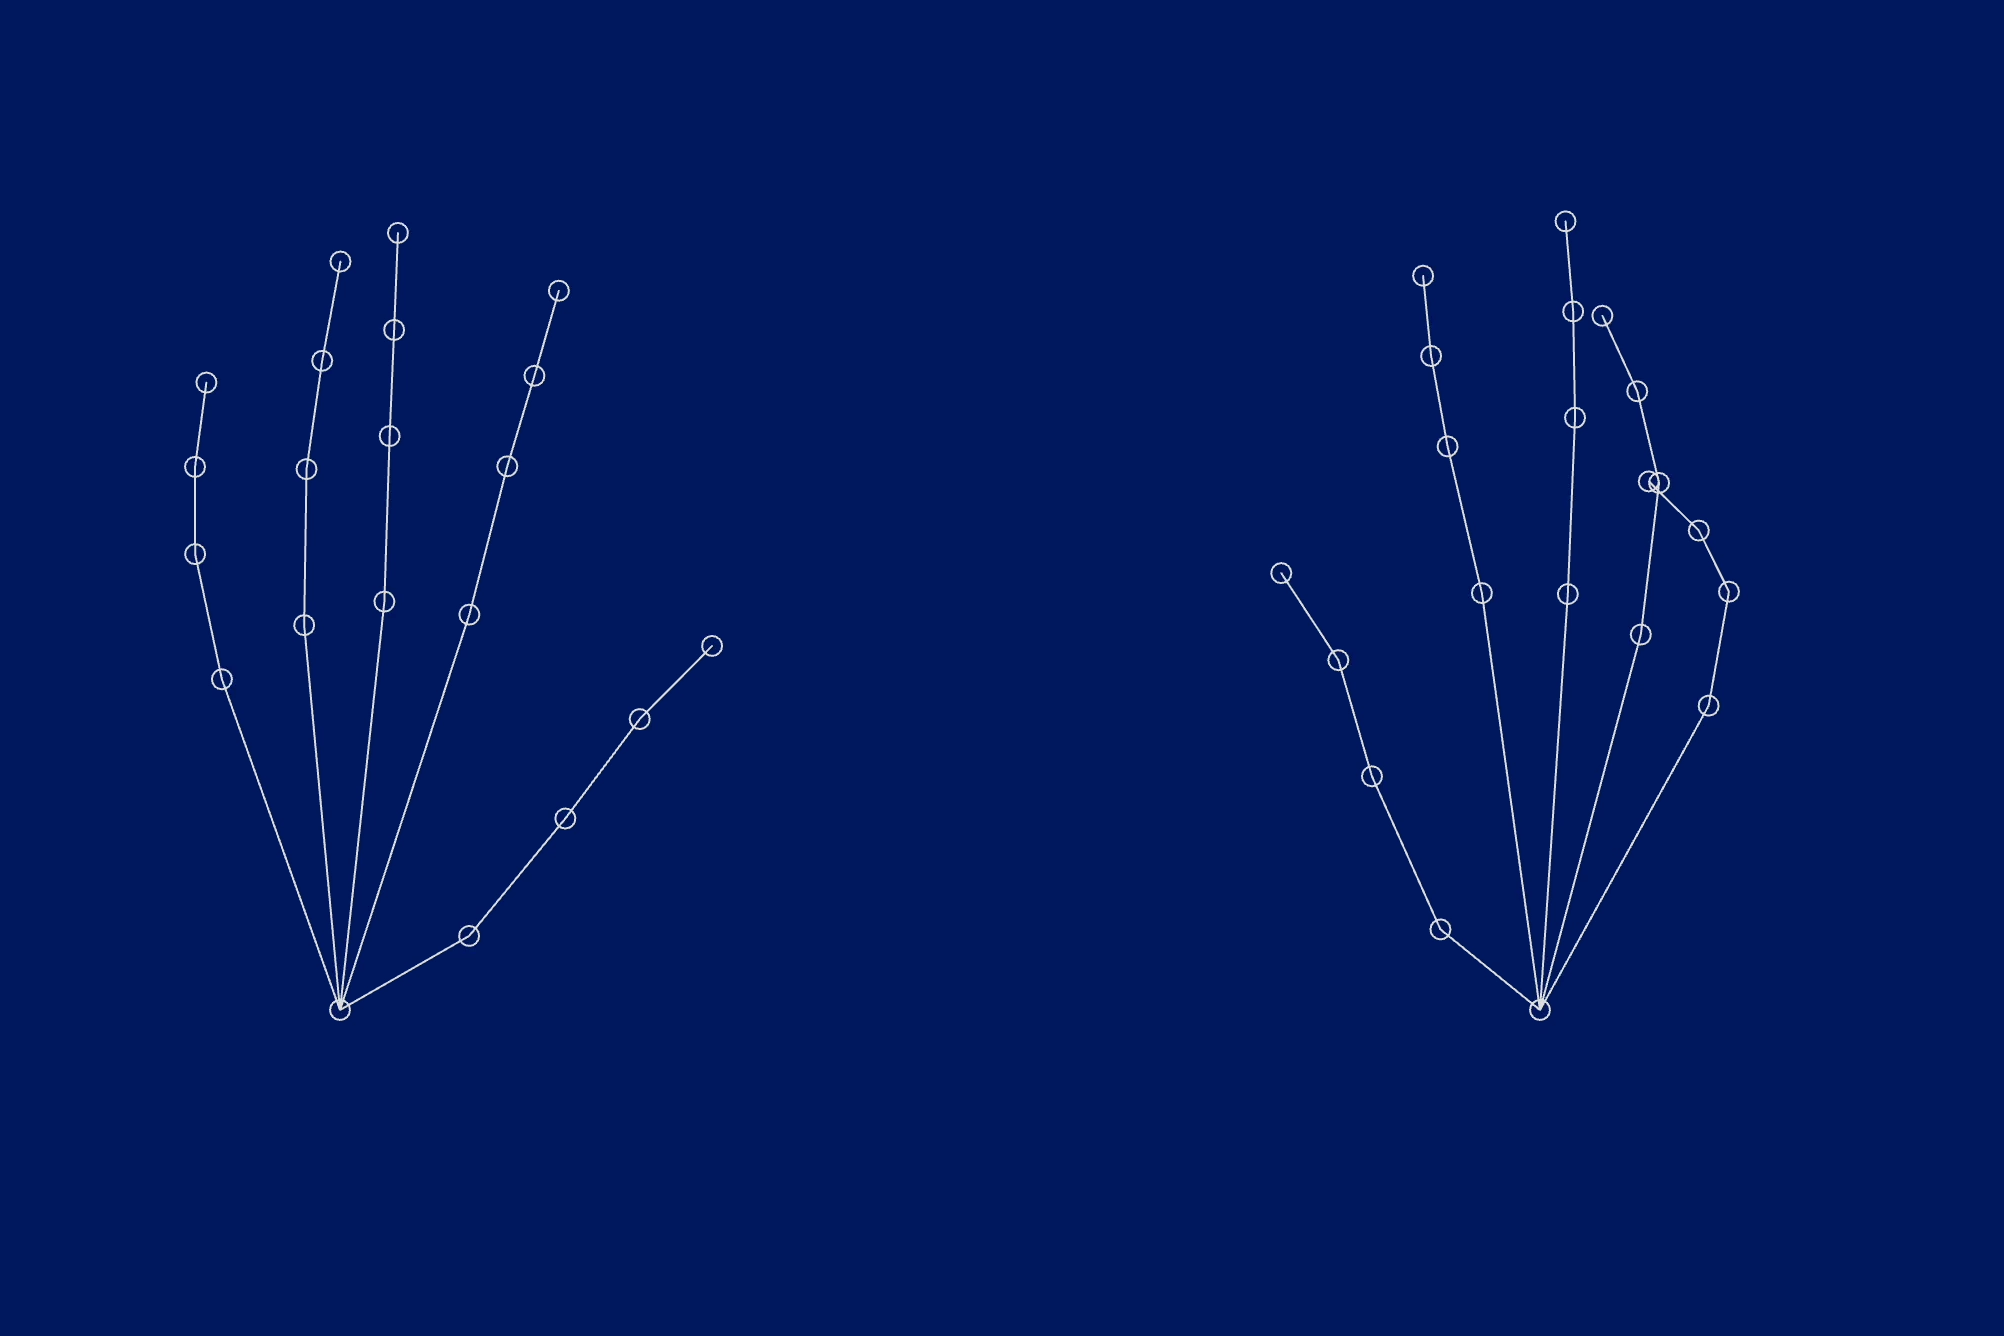
\includegraphics[keepaspectratio, width=7cm]{img/track_false.png}
    \caption{トラッキングに失敗しているとき}
    \label{fig:track_false}
  \end{minipage}
\end{figure}